\documentclass{article}

\usepackage{graphicx}
\usepackage{geometry}
\geometry{
  a4paper,
  total={170mm,257mm},
  left=20mm,
  top=20mm,
}
\usepackage{crimson}
\usepackage[T1]{fontenc}
\usepackage[round]{natbib}
\usepackage{nameref}
\usepackage{tikz}

\title{Evaluating isolation and contact tracing for control of influenza outbreaks with pandemic potential: a modelling study}
\author{Joshua W. Lambert, Authors TBC, Adam J. Kucharski}
\date{}

\begin{document}

\maketitle

\section*{Abstract}

\section*{Introduction}

Outbreaks of severe novel infectious diseases pose a major public health threat. The COVID-19 pandemic resulted in over 7 million reported deaths \citep{whocovid-19dashboardCOVID19DeathsWHO}, while the 1918 influenza pandemic caused an estimated $\sim$50 million deaths \citep{johnsonUpdatingAccountsGlobal2002}. Recent human cases of avian influenza A/H5N1, alongside transmission, illustrate the ongoing potential for viruses to infect new hosts, creating the potential for further adaption [CITE: Antia et al, Nature, 2003 + key papers on H5N1 - see my PLOS Bio piece]. It is therefore crucial to understand the effectiveness and feasibility of different intervention strategies in the face of such infections.

%Other pathogens, including those less transmissible, with longer delays between infections, and with less presymptomatic transmission, can also cause sustained outbreaks leading to the excess death of thousands \citep{whoebolaresponseteamEbolaVirusDisease2014}.  Timely and accurate response is therefore critical early in an outbreak when the pandemic or epidemic potential is still uncertain \citep{kucharskiControllingMinorOutbreaks2024}. An effective response requires understanding the efficacy and feasibility of intervention strategies across pathogens with varying epidemiological characteristics \citep{fraserFactorsThatMake2004}. \\ AK: Removed to improve flow, as this is mentioned in more detail later in intro.

The likelihood of a novel outbreak causing sustained transmission depends both the characteristics of the pathogen and its host population, as well control measures  implemented in response to early cases. A key epidemiological metric to quantify the spread of an infectious disease is the reproduction number ($R$), defined as the average number of secondary cases by a typical infectious host. If the reproduction number is greater than 1, we would expect the incidence of infections to increase over time. If $R$ is below 1, we would expect incidence to decline on average, but several cases could still occur before transmission ceases \citep{farringtonDistributionTimeExtinction1999}. Two additional factors can influence the probability a pathogen with $R$ above 1 will successfully establish within a population~\citep{lloyd-smithSuperspreadingEffectIndividual2005}. If there is a large degree of individual-level variation in transmission, the majority of infectious individuals will infect nobody, even though a minority will infect many; as a result, most newly introduced outbreaks will fail to take off. In addition, the likelihood of establishment increases if there are multiple introductions into a populations \citep{whittleOutcomeStochasticEpidemicA1955, kucharskiEarlyDynamicsTransmission2020}. \\ % AK: Note 'primary case' means first in outbreak 

Early in a novel outbreak, pharmaceutical options such as treatments and vaccines may not yet be available, leading to reliance on non-pharmaceutical interventions (NPIs) to reduce infection and disease. These interventions include individual-level targeted measures such as isolation and contact tracing, to population-level policies such as venue closures or restrictions on social mixing (Huag et al., 2020) [AK: probably a better reference out there, e.g. Sharma et al, Nature Comms]. The success of such interventions in curtailing transmission before it becomes sustained depends on several factors, including: the type of intervention, timing of introduction, and the intervention's effectiveness \citep{longiniContainingPandemicInfluenza2005}. For highly transmissible pathogens with a short generation times (e.g. pandemic influenza), incidence of new infections can grow quickly, outpacing a response. Moreover, pathogens such as influenza, which have a large proportion of onward transmission prior to symptom onset and have asymptomatic (subclinical) cases, are less easily controlled via isolation of symptomatic cases and tracing and quarantining of their contacts~\citep{fraserFactorsThatMake2004}. \\

%Isolation of symptomatic infections aims to break the chain of transmission by preventing further infection of susceptible individuals. The earlier an infectious case can be isolated, the more effective it is at averting secondary cases, with isolation prior to becoming infectious optimal. This can make it challenging to control outbreaks with symptom-based isolation, as for most pathogens infectiousness preceeds prodromal symptoms [AK: reference? This is a strong claim – best to focus on flu I think]. Quarantining contacts exposed to an infectious individuals, independent of whether they later become a case, is a control strategy to reduce transmission before or shortly after symptom onset. Contact tracing is the process of finding the contacts of infected individuals. Both isolation and contact tracing are often used NPIs to try and curtail the growth of an epidemic. Forward contact tracing asks infected individuals who they have been in contact with so their contacts can be followed-up and isolated or quarantined if needed. Isolation, quarantine, and contact tracing is a targeted approach that looks to prevent the onward transmission of an infectious disease by tackling infected individuals and their contacts \citep{ferrettiQuantifyingSARSCoV2Transmission2020, keelingEfficacyContactTracing2020}. Isolation or vaccination of traced individuals has proved widely effective in controlling different outbreaks with a variety of pathogens differing in their aetiological and epidemiological characteristics \citep{foegeSELECTIVEEPIDEMIOLOGICCONTROL1971, bellPublicHealthInterventions2004}. However, in epidemics or pandemics where the proportion of cases or contacts missed is high, either because surveillance is patchy or because the number of contacts exceeds the capacity of the system, the efficacy of contact tracing to contain an outbreak diminishes, or at worst, fails completely \citep{dhillonWhenContactTracing2018, hellewellFeasibilityControllingCOVID192020}. \\ AK: This is probably too much fundamental background for an applied journal – readers will know what isolation and contact tracing is.

Several pre-COVID-19 studies  concluded that influenza viruses cannot be controlled by isolating individuals at symptom onset and tracing their contacts, because the rate at which infected individuals become infectious and transmit is faster than the latency in the process of isolating contacts \citep{fraserFactorsThatMake2004, klinkenbergEffectivenessContactTracing2006}. However, with the recent human infections of avian influenza (A/H5N1), mostly among poultry and cattle farmers \citep{gargHighlyPathogenicAvian2025} and the longer estimates of incubation period and serial interval from historical H5N1 data \citep{Ward2024.12.11.24318702} it may be that isolation and contact tracing is able to control influenza subtypes with pandemic potential. The (antigenic) novelty of a pathogen introduced into a human population is a leading risk factor for causing a pandemic. Thus, influenza subtypes that have low levels of existing immunity in the population are probable epidemic and pandemic candidates. This is the case for H5N1 \citep{Ward2024.12.11.24318702} and H7N9 \citep{tannerPandemicPotentialAvian2015} and was the case when H1N1 caused an outbreak in 2009 \citep{fraserPandemicPotentialStrain2009}. Historically, avian influenza (H5N1 and H7N9) has had high severity (case fatality risk $\sim 35\%-55\%$), and therefore sustained transmission in a human population could have substantial mortality and morbidity implications \citep{tannerPandemicPotentialAvian2015}. \\ [AK: These headline fatality risks are likely to be biased: https://kucharski.substack.com/p/how-fatal-is-h5n1-influenza]

In this study we evaluate the effectiveness of controlling infectious disease outbreaks that exhibit influenza-like epidemiological characteristics using a mathematical model. In effect the ability to control an epidemic with isolation and contact tracing is a race between the identification and isolation of contacts and the spread of the infectious agent \citep{reyna-laraVirusSpreadContact2021}. The dogma that influenza contagion outpaces our ability to trace and isolate in time, may not hold for all pathogen subtypes with new estimates of incubation period and serial interval \citep{Ward2024.12.11.24318702}. This study looks to define the speed and effectiveness of isolation under different response delays across epidemic scenarios to inform outbreak response; quantifying the impact of reducing the delay to isolation on outbreak containment and the utility of rapid testing.

\section*{Methods}

\subsection*{Branching process model with isolation}

To assess the efficacy of isolation and contact tracing to control an outbreak of pandemic-potential influenza we used an individual-level transmision model implemented in the R package \texttt{\{ringbp\}} \citep{hellewellRingbpSimulateEvaluate2025} (Figure \ref{fig:ringbp-model}). The epidemic simulation model uses a single-type branching process with a negative binomial offspring distribution to simulate the spread of a pathogen through a population (infinite population size, without depletion of susceptibility). Influenza subtypes have shown moderate transmission heterogeneity \citep{fraserPandemicPotentialStrain2009, heComparingCOVID191918192020, Ward2024.12.11.24318702}, but evidence is limited and the negative binomial allows flexibility between highly heterogeneous and homogeneous individual-level transmission. The mean of the negative binomial offspring distribution is the basic reproduction number ($R$), and this distribution allows the model to be parameterised to capture overdispersion of transmission, in other words, some infectors are superspreaders and infect a disproportionate number of individuals \citep{lloyd-smithSuperspreadingEffectIndividual2005, kucharskiEarlyDynamicsTransmission2020}. \\

There are three categories for individuals in the simulation, with each having their own parameterisation for the negative binomial offspring distribution: 1) \textit{community} (i.e. general population), 2) \textit{isolated}, and 3) \textit{asymptomatic}. Each group have a distinct $R$ and dispersion ($k$) parameter due to the assumed differences in transmission dynamics between groups. \\

\begin{figure}[ht]
\centering
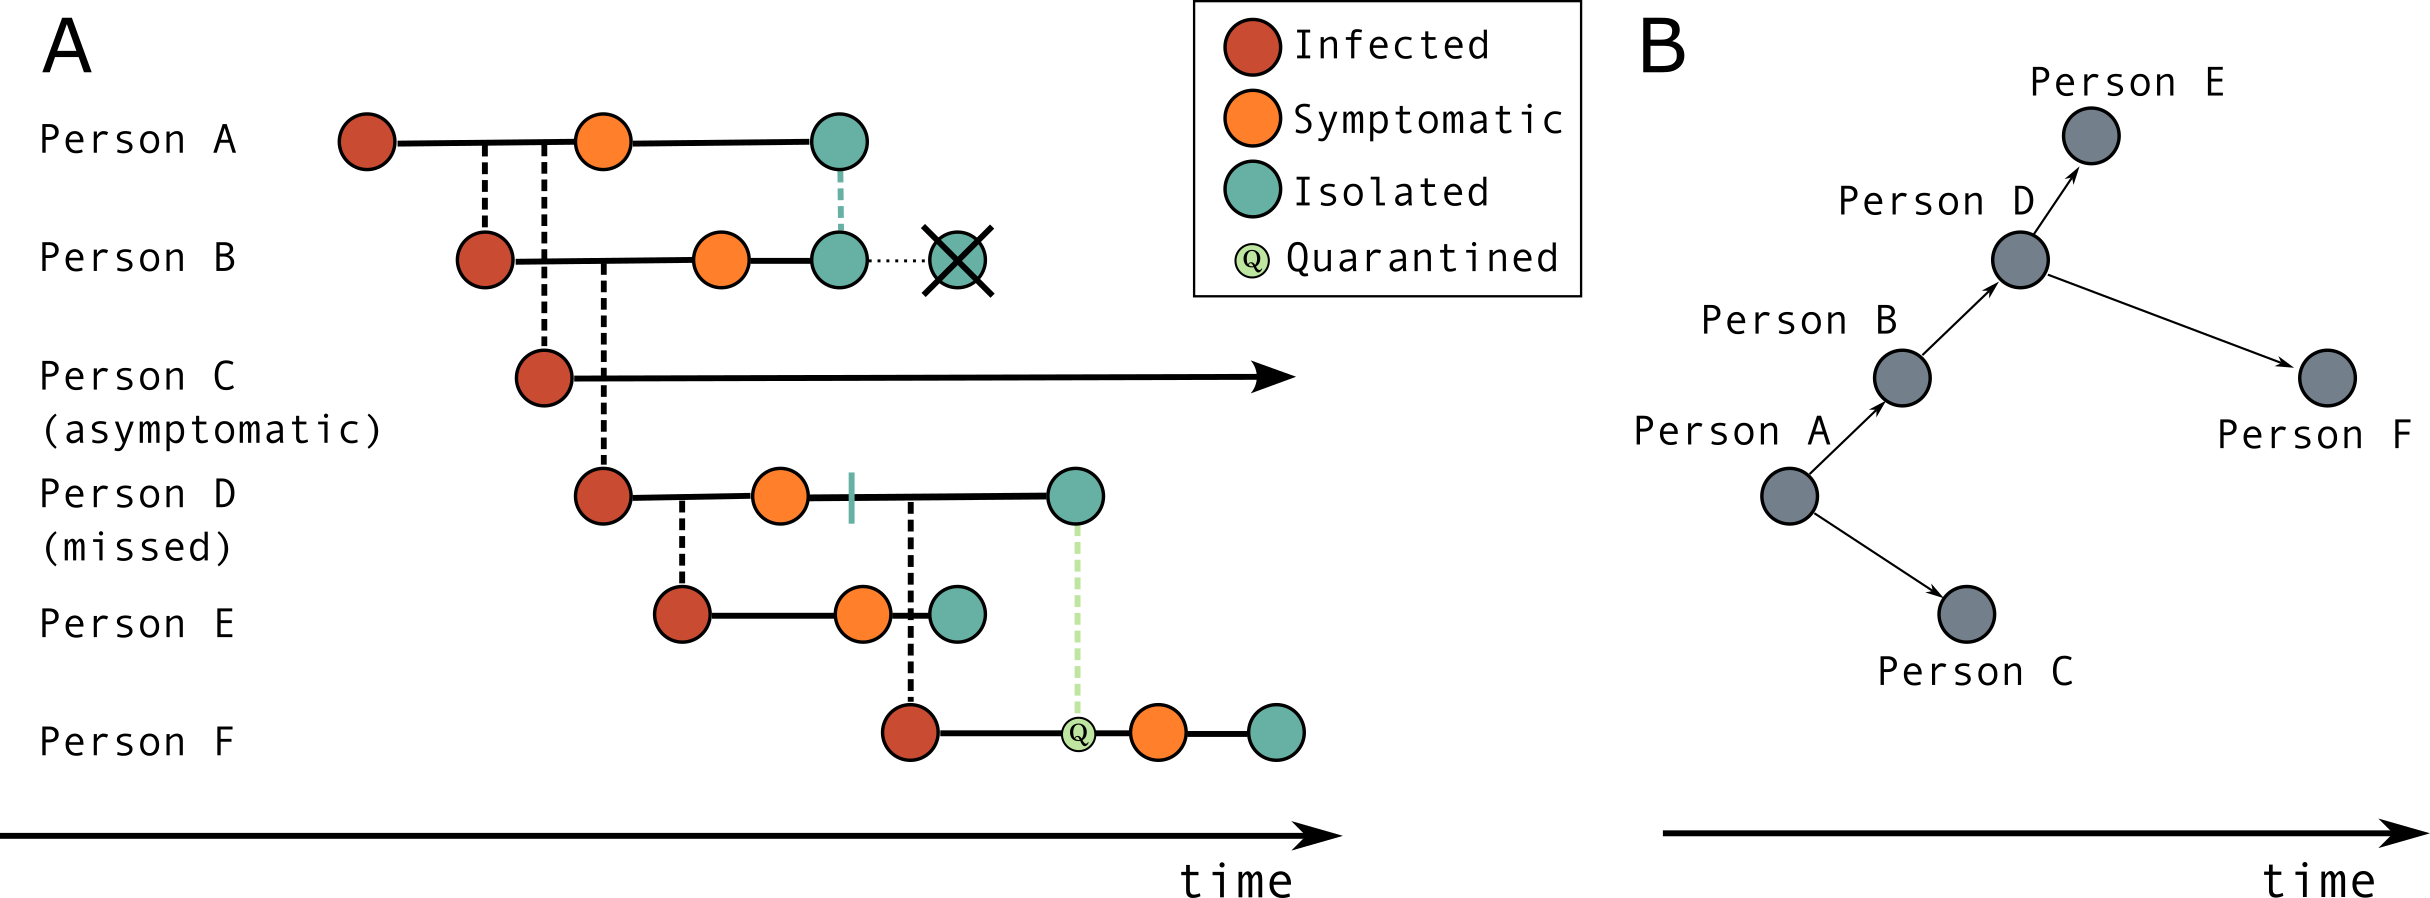
\includegraphics[width=\textwidth]{../plots/model-schematic.png}
\caption{Model schematic of the branching process with isolation, quarantine and contact tracing implemented in the \texttt{\{ringbp\}} R package. (A) The transmission chain from the index case (Person A), infection events are shown by black vertical dashed lines. The time individuals are infected is shown by the red dot, the time of symptom onset is shown by the orange dot, and the time time individuals are isolated is shown by the blue dot. Quarantine is optional in the model, assuming quarantine is active it is shown by the small green dot with a Q. The time at whcih a infectors isolation triggers the isolation of a symtomatic case is shown by the blue vertical dashed line (Person A to Person B). The isolation times that would have been triggered after a delay from symptom onset, but are after isolation was triggered by contact tracing shown by a blue dot with a cross and connected by a dotted line (Person B). Person C is an asymptomatic individual (asymptomatic cases can infect others). Person D is missed by contact tracing (contacts are traced with a probability $\rho$, and thus missed at $1 - \rho$). The time Person D would have isolated if ascertained is shown by the vertical blue mark. Assuming quarantine is active, Person F would be isolated before symptom onset at the time of the infector's (Person D) isolation time. If quarantine is not active, then Person F would be isolated after a delay from symptom onset, as they had yet to show symptoms when the infector was isolated. (B) A branching process diagram showing who-infected-whom.}
\label{fig:ringbp-model}
\end{figure}

The time between an infector being infected and then infecting an infectee (i.e. generation time) is computed using the incubation period (which samples the symptom onset time from the exposure time of each case) and sampling from a skew-normal distribution \citep{azzaliniClassDistributionsWhich1985}. This approach enables simulating transmission dynamics with a correlated structured between each case's incubation period and generation time for sensible delays between exposure, onset of symptoms, and onward transmission \citep{hellewellFeasibilityControllingCOVID192020}. This allows the proportion presymptomatic transmission to be specified, rather than defining incubation period and generation time distributions, which only indirectly allows assumptions of presymptomatic infectiousness to be derived. This simple formulation is advantageous for novel pathogens and early in outbreaks when the incubation period is estimated but the generation time is estimated with more uncertainty or unknown, and the serial interval cannot be substituted in without introducing bias \citep{brittonEstimationEmergingEpidemics2019a, lehtinenRelationshipSerialInterval2021}. \\

Given the incubation period for each case, the proportion of the infections that occur prior to, or after, the symptom onset of an infector is controlled by the parameterisation of the skew normal distribution (Figure \ref{fig:delay-distributions}C). The symptom onset time is used as the location parameter ($\xi$) of the distribution, providing the point around which the distribution is dispersed. The scale parameter ($\omega$) is fixed at 2, this parameter (with the shape parameter) defines the variance of the distribution. We select this value as it provides a realistic amount of variance when transforming onset time to exposure time (variance range for scenarios in this study: 1.5 --- 3.2). The shape parameter ($\alpha$) defines the skewness of the distribution, whereby positive values cause right-skewed values distribution around the location $\xi$, and negative values have the opposite effect (as $\alpha \rightarrow \infty$, the skew-normal converges to a folded-normal distribution). In summary, for a given parameterisation of the skew-normal distribution given the time of symptom onset ($\xi$) and fixing $\omega$ and $\alpha$ we sample the time an infectee is exposed/infected by an infector. \\

The NPI implemented in the transmission model is an isolation of symptomatic cases and contact tracing (Figure \ref{fig:ringbp-model}). When a case is symptomatic they are isolated after a delay. The timing of isolation is drawn from the onset-to-isolation distribution (see \nameref{epiparameters} section for parameterisation). Any infection times that are sampled to occur after the isolated of an infector are remove, because isolation is assumed completely effective at preventing further transmission, reducing the number of secondary cases if the speed of isolation is quicker than some or all of the secondary infection times. In other words, once a case is isolated at time $t_{isolated}$, the probability of that case infecting anyone at $t > t_{isolated}$ is zero. Another way to interpret the model is that $R$ is composed of secondary infections before isolation ($R_{pre}$) and secondary infections after an assumed isolation time ($R_{isolated}$). Symptomatic individuals that are traced are isolated either when 1) the onset-to-isolation delay after symptom onset, or 2) the infector is isolated. The isolation of the infectee is whatever occurs first of these two events.  \\

There are several mechanisms where isolation and contact tracing are imperfect at reducing onward disease transmission. The proportion of contacts missed by contact tracing is defined by the proportion of ascertainment and can range between zero, that is nobody is traced, to one, every case is traced. Symptomatic cases that have been missed when contact tracing their infectors are isolated at the onset-to-isolation delay after their symptom onset time. Additionally, contact tracing misses infections by an asymptomatic, or paucisymptomatic (subclinical), infector. In this event the infectees are missed by contact tracing owing to the infector not being known to the response system. \\

\subsection*{Defining outbreak control}

We use the same definition for outbreak control as \cite{hellewellFeasibilityControllingCOVID192020}: no new cases between 12 and 16 weeks after the start of an outbreak. The rationale for this criteria is that some outbreaks that do not take off and become large may still have a few cases for the first few weeks of an outbreak, therefore the window for control needs to be enough time after the seeding of an outbreak to be sure it is extinct. \\

There is also a maximum number of cases in simulation model, that when reached is judged to have reached a large epidemic and not controllable within 12-16 weeks. We set this limit to 500 cases. This number needs to be larger than the expected cluster size from an subcritical outbreak produce by chance (i.e. larger than $N_i / (1 - R)$, where $N_i$ is the number of initial cases and $R$ is the reproduction number).

\subsection*{Pathogen epidemiological parameters} \label{epiparameters}

In this study we evaluate the feasibility of controlling outbreaks of selected influenza subtypes that have previously caused sporadic human-to-human outbreaks with pandemic potential. We include A/H5N1, A/H1N1, and A/H7N9. These have caused outbreaks of various size and severity over the past 100 years. H5N1 has caused small outbreaks ($<$ 10 cases) of human-to-human transmission \citep{yangDetectingHumanhumanTransmission2007a, aditamaAvianInfluenzaH5N12012a}. H1N1 is now an endemic seasonal influenza with substantial population immunity, but a novel strain, H1N1pdm09, emerged in 2009 and caused a pandemic outbreak \citep{fraserPandemicPotentialStrain2009, lesslerOutbreak2009Pandemic2009}. The first human case with the H7N9 subtype was in 2013, subsequently causing five outbreak waves, but no human cases since 2019 \citep{liH7N9InfluenzaVirus2021}. Most cases are of zoonotic origin with recorded animal exposure but there have been some small clusters (2 --- 3 cases) of possible human-to-human transmission \citep{liEpidemiologyHumanInfections2014}. For the purposes of this study we assume that there is no preexisting population immunity for these influenza subtypes. This is generally true for H5N1 and H7N9 at present, and for H1N1pdm09 prior to 2009. \\

We extracted incubation periods from the epidemiological literature that have been previously estimated for the chosen Influenza subtypes. All incubation periods were found to be well described by a Weibull distribution, \cite{nishiuraEstimationIncubationPeriod2011} report the best fitting Weibull shape and scale parameters for H1N1 to be 1.77 and 1.86, respectively (Figure \ref{fig:delay-distributions}A). \cite{cowlingComparativeEpidemiologyHuman2013} report the incubation period for H5N1 and H7N9, both Weibull distributed. For H5N1 the Weibull distribution has a mean of 3.3 days and standard deviation (SD) of 1.5 days, for H7N9 the Weibull distribution has a mean of 3.1 days and SD 1.4 days \citep{cowlingComparativeEpidemiologyHuman2013} (Figure \ref{fig:delay-distributions}A). Comparatively, the incubation period for H1N1 is noticably shorter than the other two subtypes (H5N1 and H7N9), which are similar, with H5N1 having a slightly longer median (Figure \ref{fig:delay-distributions}A).  \\

The reproduction number ($R$) use to simulate transmission for each influenza subtype was 1.1, 1.5, 2.5 and 3.5. We chose these values and they represent either similar values to previously estimated $R$ values for influenza outbreaks \citep{fergusonStrategiesMitigatingInfluenza2006}, including H1N1 \citep{fraserPandemicPotentialStrain2009, lesslerOutbreak2009Pandemic2009}, or they represent an inflated values of current estimates of H5N1 and H7N9 subtypes to evaluate the effectiveness of isolation and contact tracing in the event that pathogen evolution (e.g. genetic reassortment (Peacock et al., 2025) or mutations in receptor binding preference (Lin et al., 2024)) enhances the human-to-human transmissibility of these pathogens. Current estimates for H5N1 and H7N9 subtypes are below unity (i.e. $R < 1$) (\citealt{tannerPandemicPotentialAvian2015}; \citealt{Ward2024.12.11.24318702}, but see \citealt{yangDetectingHumanhumanTransmission2007a} for a H5N1 $R$ estimate above 1) so transmission is expected to stop without intervention; with most outbreaks being small except in rare instances of superspreading events. Therefore evaluating isolation and contact tracing requires simulating outbreaks that have pandemic potential with exponential spread in the absence of control measures.

\begin{figure}[ht]
\centering
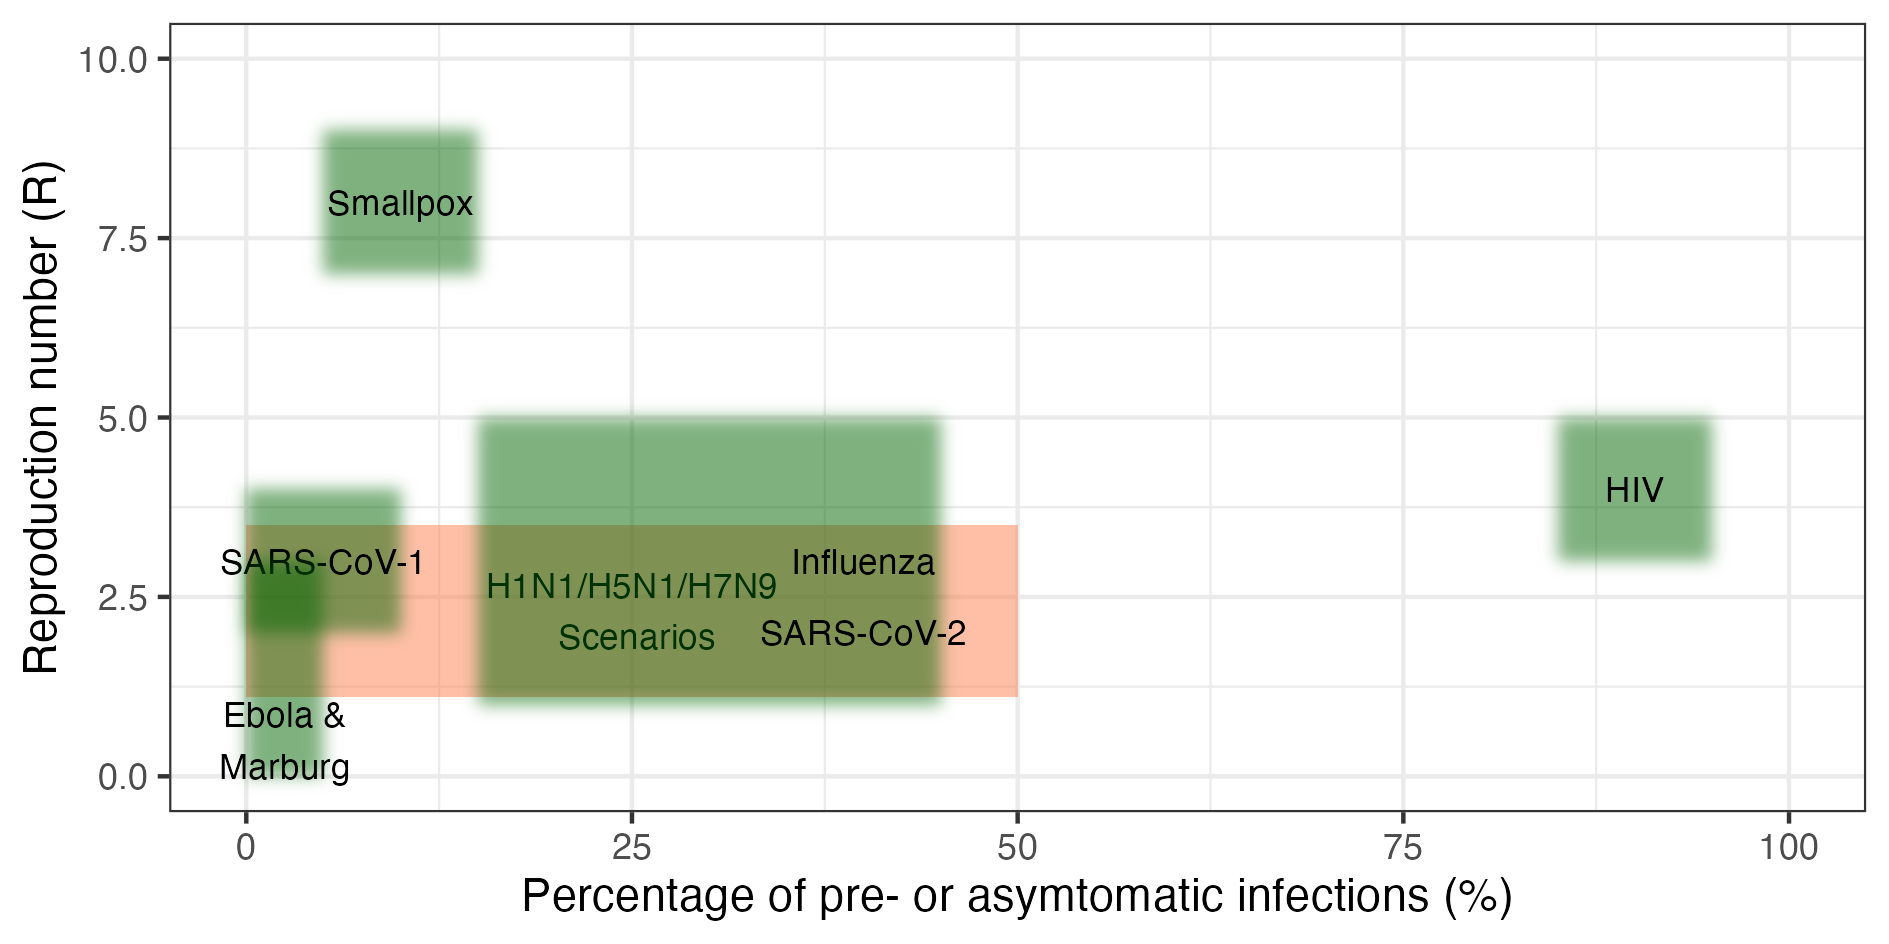
\includegraphics[width=\textwidth]{../plots/patho_param_space.png}
\caption{The pathogen characteristics, in terms of tranmissibility ($R$) and proportion of disease transmission that occurs before the onset of symptoms (including cases that are entirely asymptomatic). The figure includes: Influenza, SARS-CoV-1, SARS-CoV-2, Smallpox, Ebola, Marburg, and HIV shown by green shaded areas. The size of the shaded area reflects the differences in pathogen characteristics, both between variants and outbreaks, the blurred edges reflects uncertainty in parameter estimates. The parameter space of transmissibility and pre- and asymptomatic transmission explored in this paper is shown in the orange box.}
\label{fig:patho-param-space}
\end{figure}

\begin{figure}[ht]
\centering
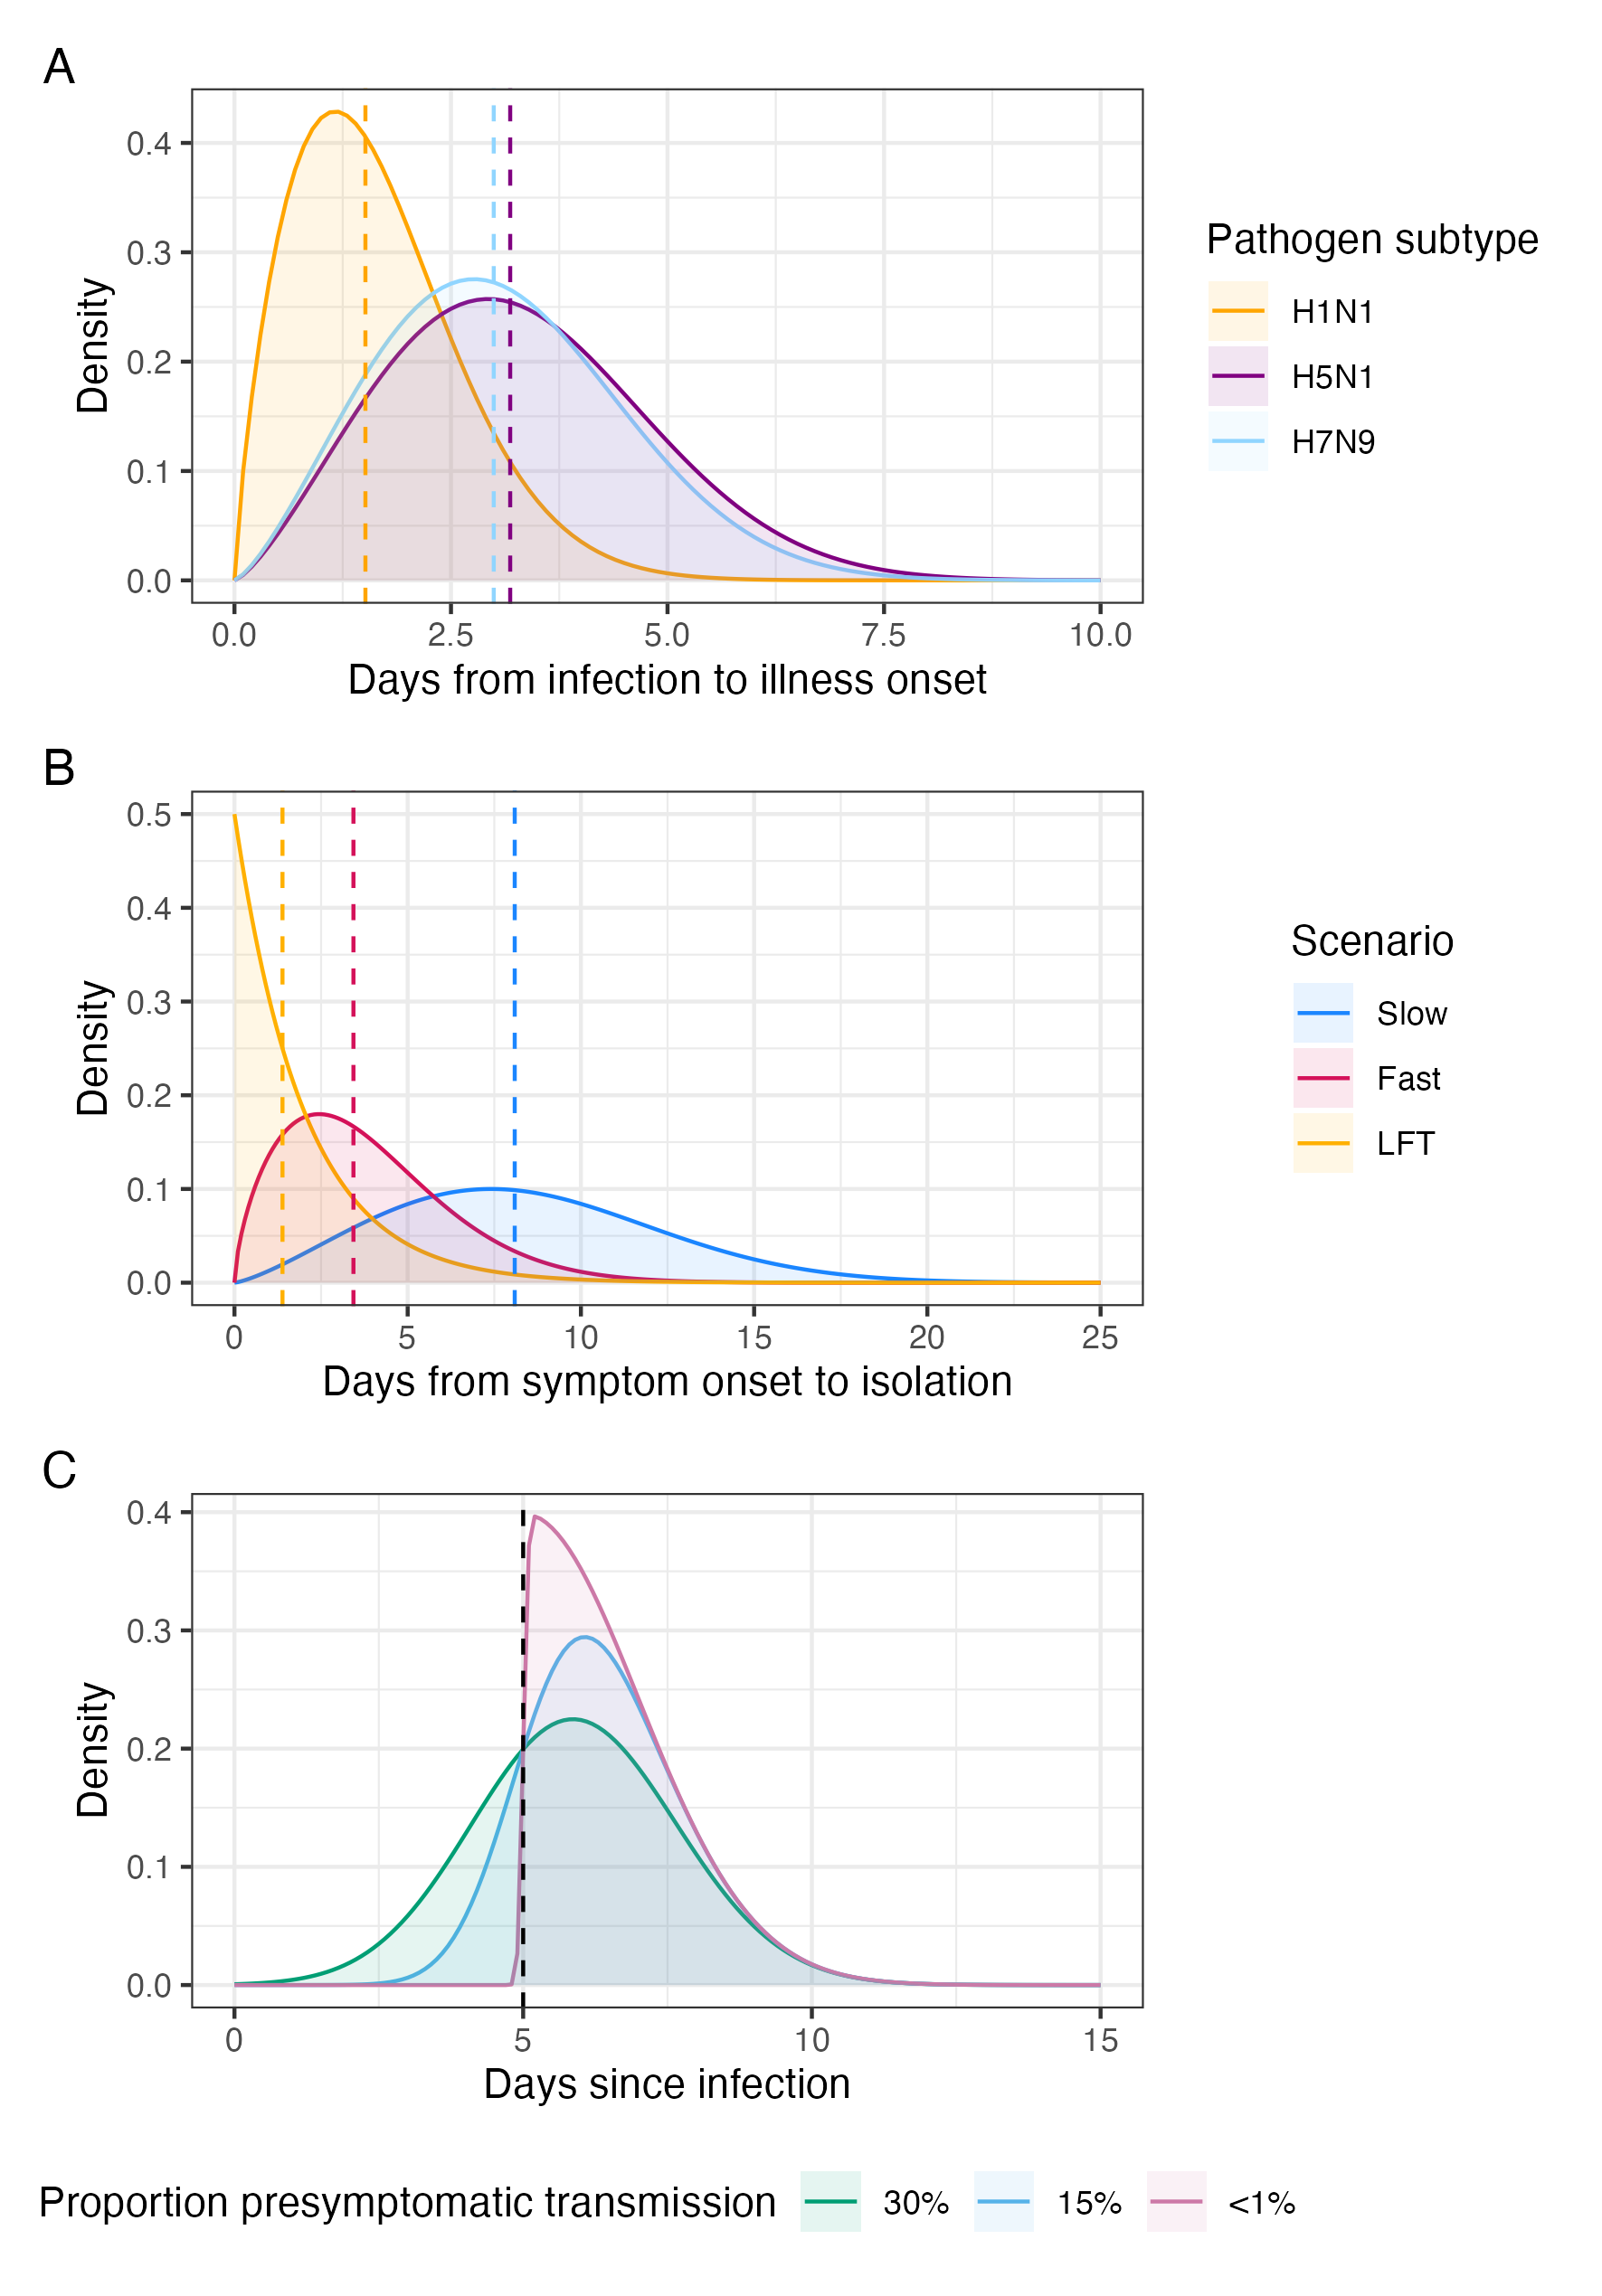
\includegraphics[width=\textwidth,height=0.85\textheight]{../plots/delay_distributions.png}
\caption{(A) Incubation period for the Influenza subtypes: H1N1, H5N1 and H7N9. (B) Three assumed onset-to-isolation delays used in the simuluation experiment. The \textit{Slow} scenario is based on the onset-to-isolation for the SARS-CoV-2 response in Wuhan, China \citep{liEarlyTransmissionDynamics2020}, the median onset-to-isolatiojn is 8.1 days (blue dashed line). The \textit{Fast} scenario is based on the onset-to-isolation for SARS-CoV-1 response in Hong Kong \citep{donnellyEpidemiologicalDeterminantsSpread2003a}, the median onset-to-isolation time is 3.4 days (red dashed line). The lateral flow test (LFT) scenario is an assumed distributed for rapid self-administered home testing upon isolation, the median delay from symptom onset to isolation in this scenario is 1.4 days (orange dashed line). (C) Proportion of presymptomatic transmission determined by the incubation period, here assumed to be 5 days (dashed vertical line), controlled by a skew-normal distribution.}
\label{fig:delay-distributions}
\end{figure}

\clearpage

\subsection*{Simulation scenarios}

To assess under what scenarios pandemic-potential influenza outbreaks could be contained with the use of isolation and contact tracing we set up a simulation experiment. We defined a parameter space to explore across a variety of epidemiological characteristics (as defined in \nameref{epiparameters} section), contact tracing effectiveness, proportion of aysmptomatic cases and presymptomatic transmission, and number of initial cases. \\

The ability to contain an outbreak by isolating infected individuals is highly contingent on the response time, or delay, between individuals becoming symptomatic, getting tested, the test results being returned and going into isolation. The probability that this series of steps will take an given amount of time is encapsulated in the onset-to-isolation delay distribution, i.e. onset-to-isolation distribution determines the time between a case developing symptoms and then becoming isolated. Here we define the onset-to-isolation as a response time as it is determined by the time delay between an individual responding to symptoms by getting tested and the turn around time for the tests to be analysed and the result returned. We view the onset-to-isolation as a feature of the public health outbreak response rather than an epidemiological characteristic of a disease. As such it is possible for pandemic response to adapt their response time to meet the needs of an outbreak. \\

We assume that an isolated case cannot transmit, so isolation is assumed to be 100\% effective once enacted ($R_{isolated} = 0$). The onset-to-isolation delay is parameterised with three scenarios: a fast response, based on the SARS in Hong Kong (Donnelly et al. 2003) and a slower response based on COVID-19 in Wuhan, China (Li et al. 2020) (Figure \ref{fig:delay-distributions}B). Both the fast and slow onset-to-isolation are parameterised as Weibull distributions, the SARS-like distribution has shape ($\lambda$) 1.65 and scale ($k$) 4.29 (mean = 3.83 days, SD = 2.38 days), the COVID-like distribution has shape = 2.31 and scale = 9.48 (mean = 8.40, SD = 3.87 days) (Figure \ref{fig:delay-distributions}B). These two empirically informed delay distributions provide a guide to possible response times in the case of an influenza outbreak and will enable us to evaluate if such delays are too long to contain a disease that can transmit rapidly such as influenza. We also include a third onset-to-isolation scenario based on the case where lateral flow rapid tests (LFTs) are provided to all individuals in the susceptible population and these people are freely able to self-test if they suspect they are symptomatic. We parameterise this as an exponential distribution, with rate ($\lambda$) 0.5, where most individuals will self-test very shortly after they become symptomatic (approximately 40\% of cases will self-test within the first day of sympmtom onset), with a few people waiting a 2 or more days before testing (approximately 3\% take longer than one week to take a self-test). We assume that LFTs are 100\% accurate so all symptomatic individuals will receive a positive test result. \\

We define the proportion of presymptomatic transmission ($\theta$) follwowing the approach of \cite{hellewellFeasibilityControllingCOVID192020} by parameterising a skew-normal distribution to sample the infection times using the incubation period and a shape parameter ($\alpha$). The shape parameter controls the proportion of presymptomatic transmission by modulating the proportion of tranmission times that are less than the incubation time (Figure \ref{fig:delay-distributions}C). We parameterise the skew-normal with three proportion of presymptomatic transmission scenarios: <1\%, 15\%, 30\%, these correspond to $\alpha$ values of 30, 1.95 and 0.7, respectively (Figure \ref{fig:delay-distributions}C). Therefore, in all scenarios most transmission occurs after symptom onset, but due to isolation only impacting symptomatic individuals the greater proportion of transmission that occurs before symptom onset, the less effective isolation and contact tracing is hypothesied to be. \\

The proportion of pandemic-potential influenza infections that are asymptomatic varies for past outbreaks. There is evidence from past human outbreaks of H1N1pdm and H5N1 (2.3.4.4b) that some laboratory (polymerase chain reaction) positive cases showed no symptoms or symptoms too mild to be considered influenza-like illness \citep{lesslerOutbreak2009Pandemic2009, gargHighlyPathogenicAvian2025}; but whether human-to-human transmission can occur while subclinical is unknown. There is no evidence of asymptomatic transmission for the H7N9 subtype \citep{xuSerologicalInvestigationSubclinical2013}. Here we assume that asymptomatic cases occur and can infect others, but are uncommon and that the majority of cases will develop symptoms during their infectious period.  We ran three scenarios, one with zero asymptomatic illness, another with 10\% of cases being asymptomatic and the most extreme scenario where 30\% of cases never develop symptoms and thus are not isolated and secondary cases are missed by contact tracing. \\

The feasibility of epidemic containment by contact tracing is expected to depend on the proportion of close contacts of cases that are traced and isolated if symptomatic. We varied the proportion of contacts ascertained in the model between 0 and 1, at intervals of 0.2. In cases when the proportion of contacts traced is zero, isolation after the delay from symptom onset is the only NPI reducing disease transmission. To test scenarios where an outbreak starts with different number of initial infections, we simulate with either 5, 20 or 40 initial indepedent cases. This could represent importation of multiple cases in a single event, such as a flight with multiple positive cases. \\

We fixed some parameters across all simulations. The dispersion parameter for the negative binomial offspring distribution was fixed at 1 for isolated cases, and 0.16 for subclinical and community cases. For computational efficiency we capped the maximum number of days the simulation could run for to 365. This is substantially longer than the 12-16 week window for evaluating outbreak control so does not influence the results. Additionally, we limit simulations to 500 cases. This is an arbitrary threshold we judge to be large epidemic that is not controllable.

\section*{Results}

The ability to control an influenza epidemic is highly dependent on the reproduction number and the speed of isolation after symptom onset (Figure \ref{fig:prop-outbreak-control-R}). A higher outbreak reproduction number results in a smaller percentage of outbreaks controlled at a given percentage of contacts traced, except in cases where they are equal because zero or all outbreaks are contained, across all onset-to-isolation scenarios (Figure \ref{fig:prop-outbreak-control-R}). When the reponse to isolate cases is slow then outbreaks with $R = 1.5$ require at least 50\% of contacts traced to contain at least half of simulated outbreaks. When $R$ is 2.5 or 3.5 then contact tracing needs to be extremely comprehensive ($>90\%$) to have a chance at containment, and even then $R = 3.5$ influenza outbreaks on average are uncontrolled (Figure \ref{fig:prop-outbreak-control-R}A). Especially for H1N1, given its faster tempo of transmission, has a much lower probability of containment at 100\% of contacts traced with a slow, COVID-19-like, isolation response time (Figure \ref{fig:prop-outbreak-control-R}A). In a scenario with a fast, Hong Kong SARS-like, onset-to-isolation response, outbreaks with $R = 1.1$ are almost always contained at any proportion of contacts traced (Figure \ref{fig:prop-outbreak-control-R}B). For slow and fast isolation response delays there is a substantial difference between outbreaks with a $R$ slightly above unity ($R = 1.1$) which were controlled at a low levels ($\geq 20\%$) of isolation and contact tracing for all three influenza subtypes (Figure \ref{fig:prop-outbreak-control-R}A,B). As $R$ increases to 1.5 there is a dramatic decline in the ability to control the epidemic without isolation of traced contacts (i.e. 0\% contact ascertainment), however, outbreaks with $R = 1.5$ are mostly contained once the percentage of contacts ascertained in tracing exceeds 50\% (Figure \ref{fig:prop-outbreak-control-R}B). For more transmissible influenza scenarios, even a fast isolation response, with an average of 3.4 days between symptom onset and isolation, requires $>70\%$ of contacts traced for most outbreaks to be controlled (Figure \ref{fig:prop-outbreak-control-R}B). \\

The most rapid scenario we simulated to emulate individuals self-testing with LFTs, has the same trend of increased chance of outbreak containment by reducing the time between symptom onset and isolation, as the slow and fast scenarios (Figure \ref{fig:prop-outbreak-control-R}). The contol of low transmissible ($R \in {1.1, 1.5})$ influenza pathogens is almost always guranteed even in the absence of contact tracing and only isolating cases immediately if positive on an LFT (Figure \ref{fig:prop-outbreak-control-R}C). Assuming ubiquitous access to home testing and that 63\% of symptomatic cases test and isolate within the 24 hours symptom onset, 75\% ascertainment of contacts results in most outbreaks controlled for all influenza transmissibility scenarios ($R \leq 3.5$). The LFT isolation strategy is also the only onset-to-isolation delay which can achieve 100\% of outbreaks controlled when all contacts are traced (Figure \ref{fig:prop-outbreak-control-R}C). \\

The difference in influenza subtype incubation period influences the efficacy of isolating and tracing. This effect is most pronounced when the percentage of outbreaks controlled is greater than 0\% and less than 100\% (i.e. not at the boundary) (Figure \ref{fig:prop-outbreak-control-R}). The shortest incubation period, H1N1, is predominantly the least controllable for a given reproduction number, showing that infections that are symptomatic shortly after infection and in some instances transmission while subclinical limit our ability to effectively trace and isolate their potential infectees in time to prevent disease transmission. The variance between the influenza subtypes at each percentage of contacts traced and isolated varies (i.e. difference between circle, triangle and square points at each contacts traced \% in Figure \ref{fig:prop-outbreak-control-R}). This variance is greatest at intermediate (20\% - 80\%) contact tracing effectiveness and intermediate values of $R$ (1.5 and 2.5) (Figure \ref{fig:prop-outbreak-control-R}). This could indicate a substantive role for incubation period durartion in the control of disease transmission. However, this variance in proportion of outbreaks controlled between pathogen subtypes does not show a strong pattern across all scenarios simulated (Figure \ref{fig:prop-outbreak-control-var-R}). There is a weak pattern of increased variance in controllability between subtypes at intermediate values of $R$, overall it seems that incubation period causes differences in control-by-isolation effectivness when not at the boundary of epidemic controllability. In other words, differences between influenza subtypes arise when not in a situation of high transmissibility and low contact tracing effectivness that cannot contain any outbreaks, nor low transmissibility and high contact tracing effectivenss easily contain all outbreaks (Figure \ref{fig:prop-outbreak-control-var-R}). \\

\begin{figure}[ht]
\centering
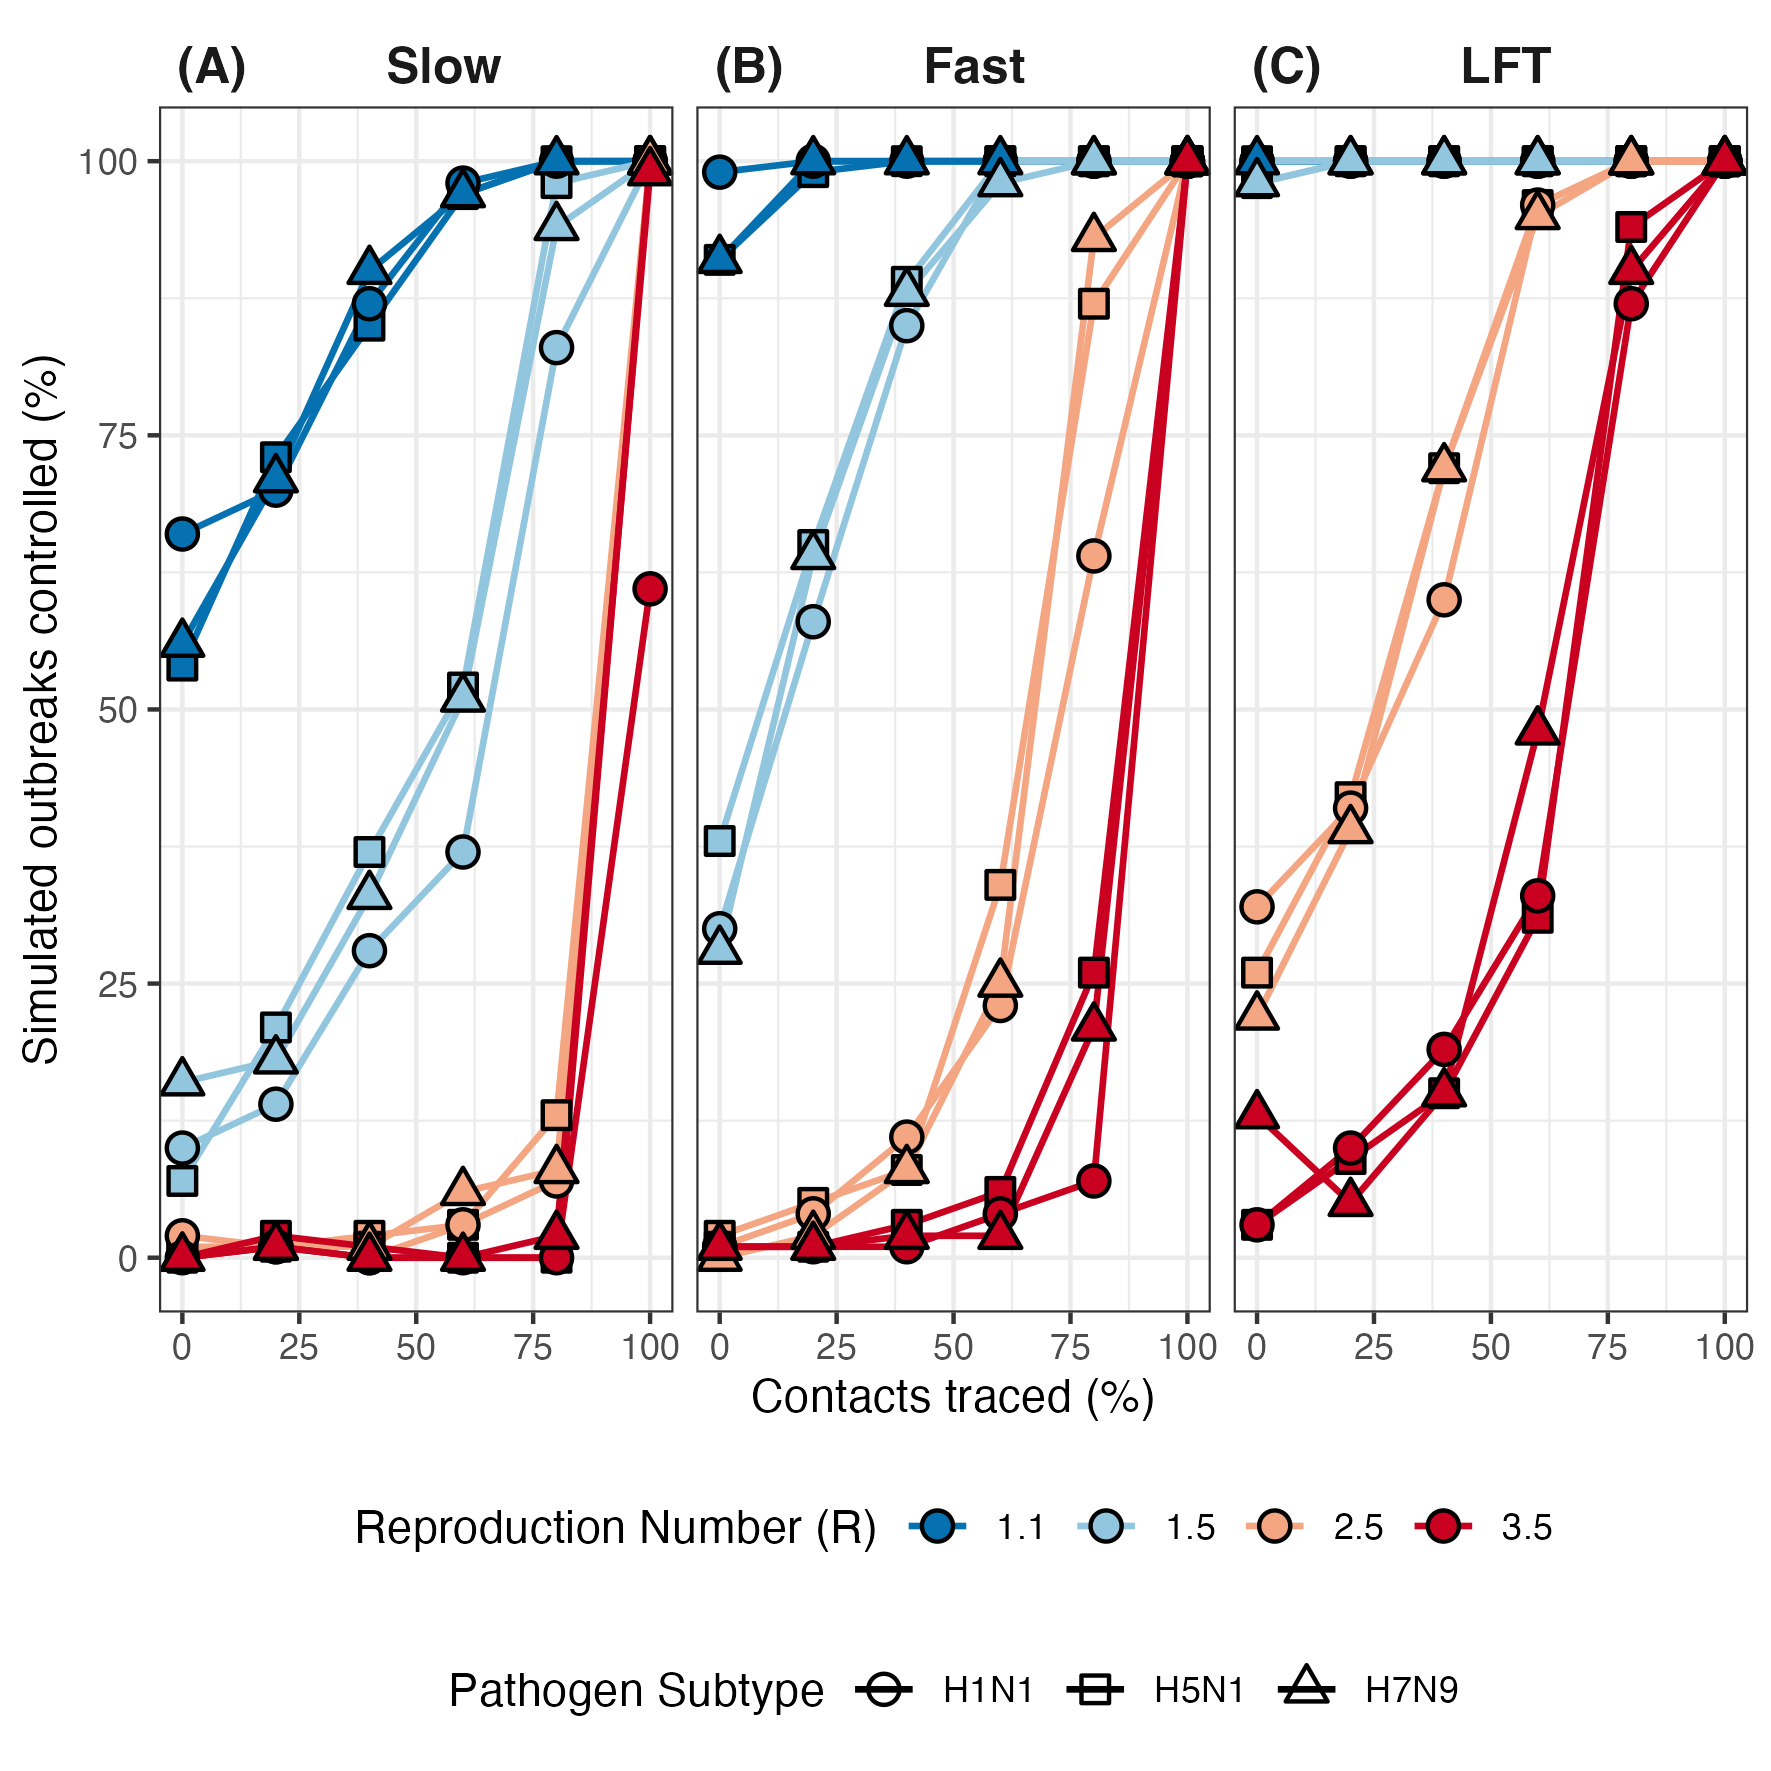
\includegraphics[width=\textwidth]{../plots/prop_outbreak_control_reproduction_number.png}
\caption{The percentage of outbreaks controlled across values of isolation and contact tracing effectiveness, for outbreaks with an assumed reproduction number ($R$) of either 1.1 or 1.5. This is for a baselines scenario where the number of initial cases is 10, the proportion of presymptomatic transmission is 15\%, all cases are assumed symptomatic, and the onset-to-isolation delay is assumed to be SARS-like.}
\label{fig:prop-outbreak-control-R}
\end{figure}

\clearpage

The proportion of transmission that occurs before on the onset of symptoms has a moderate affect on epidemic containment for across isolation response rates (Figure \ref{fig:prop-outbreak-control-prop-presym-iso}). In all scenarios decreasing the proportion of presympatomatic transmission result in an greater or equal probability of outbreak control. When presymptomatic transmission is minimal, most $R = 1.1$ outbreaks go extinct without any contact tracing, at any rate of isolation after symptom onset, with extinction ensured if isolated after LFT testing (Figure \ref{fig:prop-outbreak-control-prop-presym-iso} leftmost column). Furthermore, when  $<1\%$ of transmission is presymptomatic, rapidly isolating after symptoms (e.g. after self-testing) can contain more than half of outbreaks for all transmissibility scenarios ($R \leq 3.5$) (Figure \ref{fig:prop-outbreak-control-prop-presym-iso}). Conversely, when 30\% of transmission is presymptomatic, less than half of highly transmissible epidemics are controlled, even with the most optimistic isolation response time and contact tracing coverage (Figure \ref{fig:prop-outbreak-control-prop-presym-iso} rightmost column). \\

The pattern of outbreak control is broadly similar between 10\% asymptomatic cases and the 0\% and 30\% asymptomatic scenarios (Figure \ref{fig:prop-outbreak-control-prop-asym-iso}). Qualitative difference are in the 30\% asymptomatic scenario for LFT isolation, where the ability to control highly transmissible influenzas reduces to less than a quarter of outbreaks controlled at maximum contact tracing coverage (Figure \ref{fig:prop-outbreak-control-prop-asym-iso}). When every case is symptomatic the likelihood of containing highly transmissible outbreaks drastically increases for all onset-to-isolation response delays (Figure \ref{fig:prop-outbreak-control-prop-asym-iso}). \\

The ability to control an epidemic that can readily transmit human-to-human is moderated by the initial number of infectious individuals that seed the outbreak. The higher the number of cases the less chance that stochastic extinction of a transmission chain will end the whole epidemic. For an influenza pandemic, the number of initial infected individuals influences efficacy of control-by-isolation at all transmissibility scenarios evaluated ($R \in \{1.1, 1.5, 2.5, 3.5\}$, Figure \ref{fig:prop-outbreak-control-num-init-cases}). When $R = 1.1$ most outbreaks can be controlled without isolation and contact tracing, even with 40 initial infectors Figure \ref{fig:prop-outbreak-control-num-init-cases}). When $R = 1.5$ the increase in the number of initial infections from 5 to 20 has a large decrease in outbreaks controlled at low levels of contact tracing, the same pattern when the number of initial infectors is twofold larger at 40, but these differences in outbreak control diminish as contact tracing increases towards 100\% (Figure \ref{fig:prop-outbreak-control-num-init-cases}). When the number of cases seeding the outbreak is $\geq 20$ at $R = 2.5$ a large proportion of outbreaks become uncontrollable until contact tracing reaches $\geq 80\%$. In the worst case transmissibility scenario ($R = 3.5$) if contact tracing is not activated until at least 20 individuals are infected then close to 100\% of contacts with need to be traced in order to control the majority of outbreaks; except for H1N1 where only 25\% of outbreaks are controlled if seeded with 40 cases (Figure \ref{fig:prop-outbreak-control-num-init-cases}).  \\

\begin{figure}[ht]
\centering
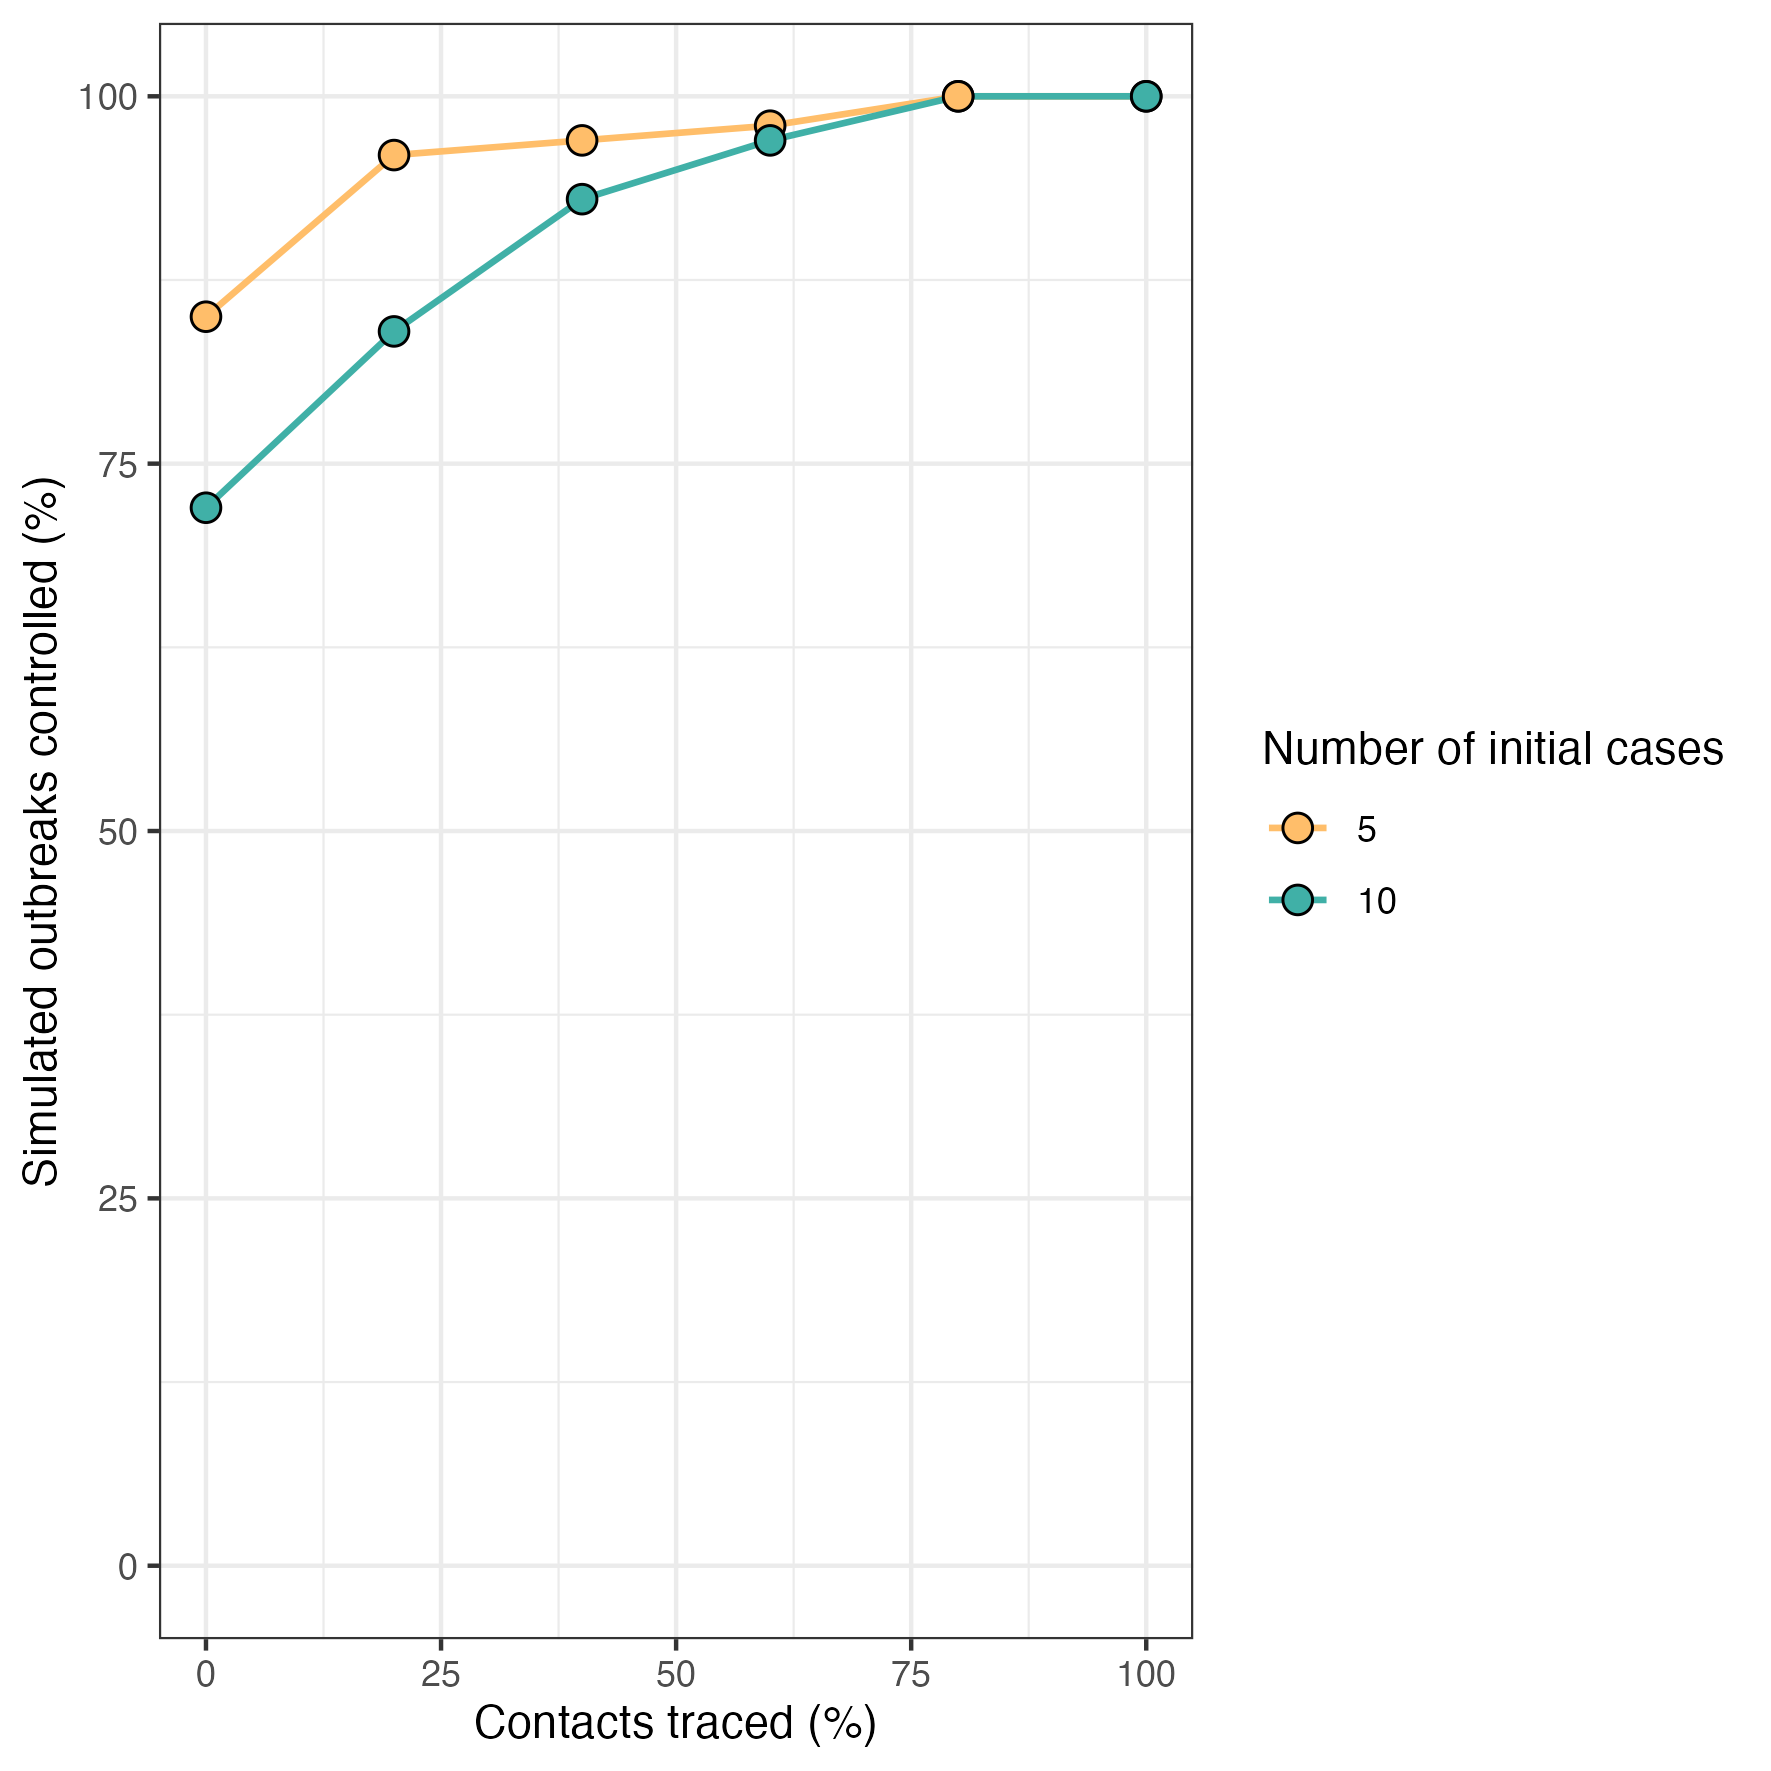
\includegraphics[width=\textwidth]{../plots/prop_outbreak_control_num_init_cases.png}
\caption{The percentage of outbreaks controlled across values of isolation and contact tracing effectiveness, for outbreaks with an initial number of seeding infections assumed to be either 5 or 10. This is for a baselines scenario where the reproduction number is 1.5, the proportion of presymptomatic transmission is 15\%, all cases are assumed symptomatic, and the onset-to-isolation delay is assumed to be SARS-like.}
\label{fig:prop-outbreak-control-num-init-cases}
\end{figure}

\clearpage

The median size of contained influenza outbreaks is predominantly below 100 cases for all influenza subtypes and isolation response delays (Figure \ref{fig:median-controlled-outbreak-size}). There are a few parameter sets that have a median cumulative outbreak size between 200 --- 400, but very few have 400 --- 500. This elucidates that when an outbreak is eliminated by isolation alone or in combination with contact tracing across ascertainment levels, it is done so with a relatively small number of cases (Figure \ref{fig:median-controlled-outbreak-size}). The total size of controlled outbreaks is also relatively constant across influenza subtypes and isolation response (Figure \ref{fig:median-controlled-outbreak-size}), noting that that the percentage of controlled outbreaks between parameter sets varies drastically with some only producing uncontrolled outbreaks (Figure \ref{fig:prop-controlled-outbreak}, \ref{fig:prop-outbreak-control-R}). \\

Contact tracing systems have a capacity limit which if exceeded will lower ascertainment of case contacts. The infinite susceptible population assumption in our model means uncontrolled outbreaks and contacts requiring tracing can become infinitely large. However, we find that in the early acute phase of both contained and uncontained epidemics the maximum weekly cases exceeds 600 in some scenarios (Figure \ref{fig:max-weekly-cases}). These cases and their contacts require testing and potentially isolating, showing the rapid speed at which outbreaks can overburden surveillance systems. The fact that some outbreaks have more maximum weekly case than the outbreak limit we define shows that outbreaks can become almost impossible to control on the scale of weeks from the initial cases (Figure \ref{fig:max-weekly-cases}). When isolation and 100\% of contacts are traced in the most optimal isolation response scenario (LFT) the maximum number of cases weekly is around 450 ($R = 3.5$).

\section*{Discussion}

\begin{itemize}
\item This study has looked at the feasibility and effectiveness of isolation and contact tracing for influenza subtypes that have cause epidemic outbreaks.
\item Outbreaks controlled at 50\% of contacts traced and isolated is over ??\%, highlighting the effectiveness of this intervention for infectious diseases are not highly transmissible between humans.
\item Discuss the existing flu vaccines and antivirals that can be used an interventions in addition to NPIs
\item In modelling the effectiveness of isolation and contact tracing we have assumed that there is no capacity limits on contact tracing, which does not hold in large outbreaks such as SARS-CoV-2 (ref). We also ignore potential socio-political factors that would prevent health worker from visiting or contacting infected individuals or contacts of infected individuals (Dhillon and Kelly, 2018). We also did not consider zoonotic spillover infections or formite transmission.
\item Digital tracing has capacity for large-scale contact tracing (pingdemic), also rapid tests are a complementary approach for limiting spread.
\item In this study we model isolation and contact tracing as the sole intervention in containing an influenza outbreak. This is to provide an assessment of its effectiveness for rapidly transmission and potentially highly transmissible subtypes. However, in reality, pandemic preparedness to a pandemic potential influenza would not need to deploy interventions, such as contact tracing individually or sequentially, instead they can be used in combination, such as antivirals (e.g. oseltamivir), rapid tests, contact tracing, and vaccination.
\item Antivirals for half the UK, these can be deployed in rapid response to flu pandemic.
\item In this study we have parameterised the transmission model with parameter from avian influenza subtypes (H5N1 and H7N9) and a influenza subtype that caused an epidemic in the recent past (H1N1), and response delays from SARS and COVID-19 outbreaks. However, these results can be used to inform other influenza subtypes that exhibit similar epidemiological characteristics in transmissibility and severity from past outbreaks (H2N2 and H3N2) and still exist in animal reservoirs for potential spillovers back into human populations (ref).
\item This study used a branching process model to simulate individual-level transmission and intervention. The model assumes an infinite population size with no interdependence of isolation and contact tracing between cases whereby a case may be in contact with multiple infectors and only needs to be traced in time by one contact to prevent transmission, as could happened in a fixed random network transmission model. It is unlikely that this model structure difference would have a considerable different on our results for the control of disease outbreaks with contact tracing. We suppose that because our model requires isolation sampled for a single individual, our results are more conservative on the ability to control outbreaks, and that using a random network model would indicate an increased effectivness of contact tracing (Juul and Strogatz, 2023). The infinite population assumption also means that although isolated individuals are assumed to not transmit, there are always other individuals that non-isolated infectors can transmit to, whereas a fixed random network model that assumes optimal indefinite isolation will block of parts of the network and overestimate contact tracing effectiveness (Juul and Strogatz, 2023).
\item The reproduction number for H5N1 (including clade 2.3.4.4b) and H7N9 influenza subtypes have been estimated to be far below 1 (Ward et al., Garg et al., 2025). Therefore, the transmissibility scenarios explored in this study are speculative and assume that pathogen evolution increases human-to-human transmission potential. If transmissibility of these avian influenza subtypes remains constant over time then outbreaks are expected to be subcritical and will not produce epidemics and thus not require interventions. If cases of avian influenza are detected with routine surveillance without a known animal source, it may indicate sustained human-to-human transmission and can be a trigger to commence isolation and contact tracing while the number of initial cases is presumed small, which as we show increases epidemic controllability (Figure \ref{fig:prop-outbreak-control-num-init-cases}).
\item This study has evaluated the ability to control the outbreak of an infectious disease independent on its severity. Infection severity and fatality risks are of course critical when formulating a pandemic response plan. By understanding the efficacy of isolation and contact trace for a given epidemiological characterstic, outbreak mortality and morbidity can hopefully be minimised by reducing disease incidence over time to elimination.
\item Our branching process model used a simple forward contact-tracing mechanism that reduces the number of secondary contacts based on the timing of isolation of symptomatic cases. This contact tracing stragety is minimal cost and effort. In scenarios where outbreaks are uncontrolled a more comprehensive and costly contact tracing system where infectors and contacts of infectors (i.e. backward and forward contact tracing) are followed up, which has been shown to be more effective at outbreak containment (Klinkenberg et al., 2006).
\item Isolation and contact tracing complementing in combination with other quickly available measures for pandemic potential influenza strains, such as rapid testing and antivirals \citep{haydenPerspectivesAntiviralUse2001}.
\item This paper has focused on forward contact tracing. Backward contact tracing, whereby infected individuals are asked who they have been in contact with prior to being infected to identify the source of infection and potentially forward trace from the source, is applicable to infectious with long infectious periods (e.g. HIV), but is not effective for more ephemeral infections with faster transmission, as is the case for influenza.
\item Contact tracing and isolation is a targeted approach analogous to ring vaccination. It looks to prevent onward transmission by, either isolating or quarantining contacts in the case of contact tracing, or vaccinating contacts in the case of ring vaccination \citep{kucharskiEffectivenessRingVaccination2016, whittakerQuantifyingImpactBroadly2024}. Ring vaccination for an influenza outbreak would not be effective due to the generation time, proportion of presymptomatic and asymptomatic, and likelihood of geographically widespread (i.e. non-localised) transmission.
\end{itemize}

\bibliographystyle{plainnat}
\bibliography{FluTracer.bib}

\clearpage

\section*{Supplementary Material}

\setcounter{figure}{0}
\renewcommand{\thefigure}{S\arabic{figure}}


\begin{figure}[ht]
\centering
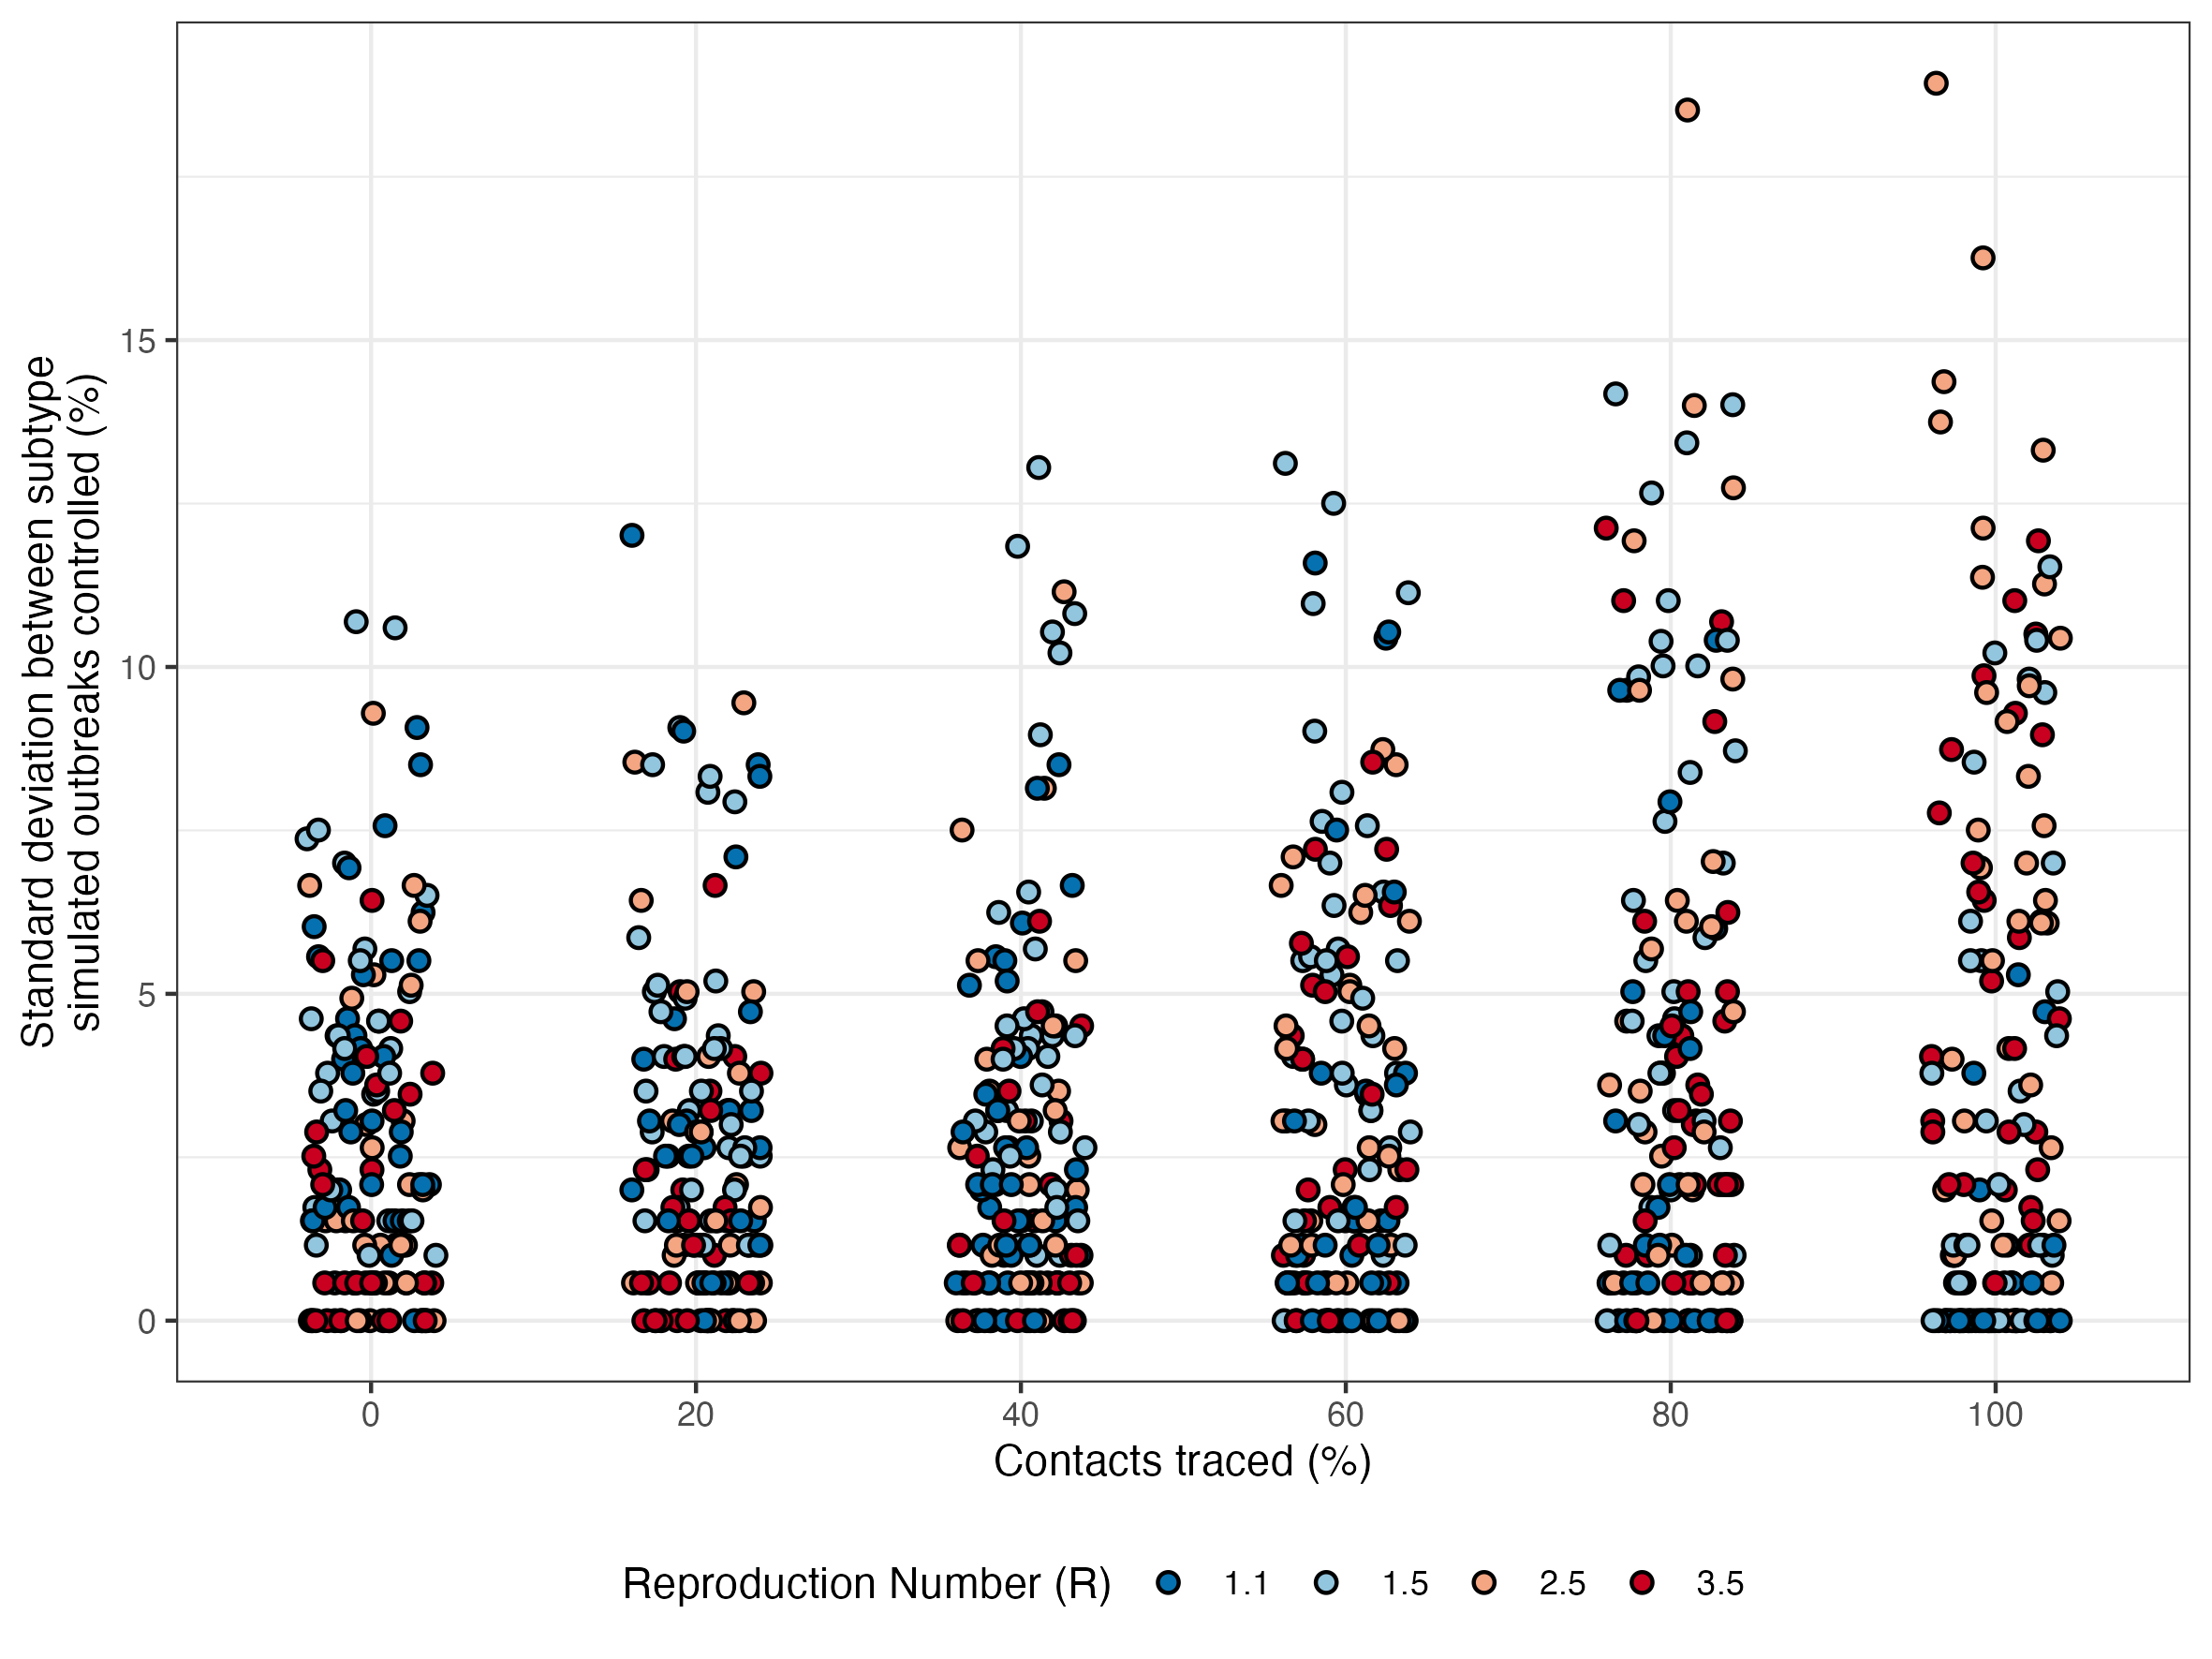
\includegraphics[width=\textwidth]{../plots/prop_outbreak_control_var_reproduction_number.png}
\caption{The standard deviation of the percentage of outbreaks controlled between influenza subtypes (H1N1, H5N1, H7N9), across percentages of contacts traced. Points are jittered horizontally reduce overlap.}
\label{fig:prop-outbreak-control-var-R}
\end{figure}

\begin{figure}[ht]
\centering
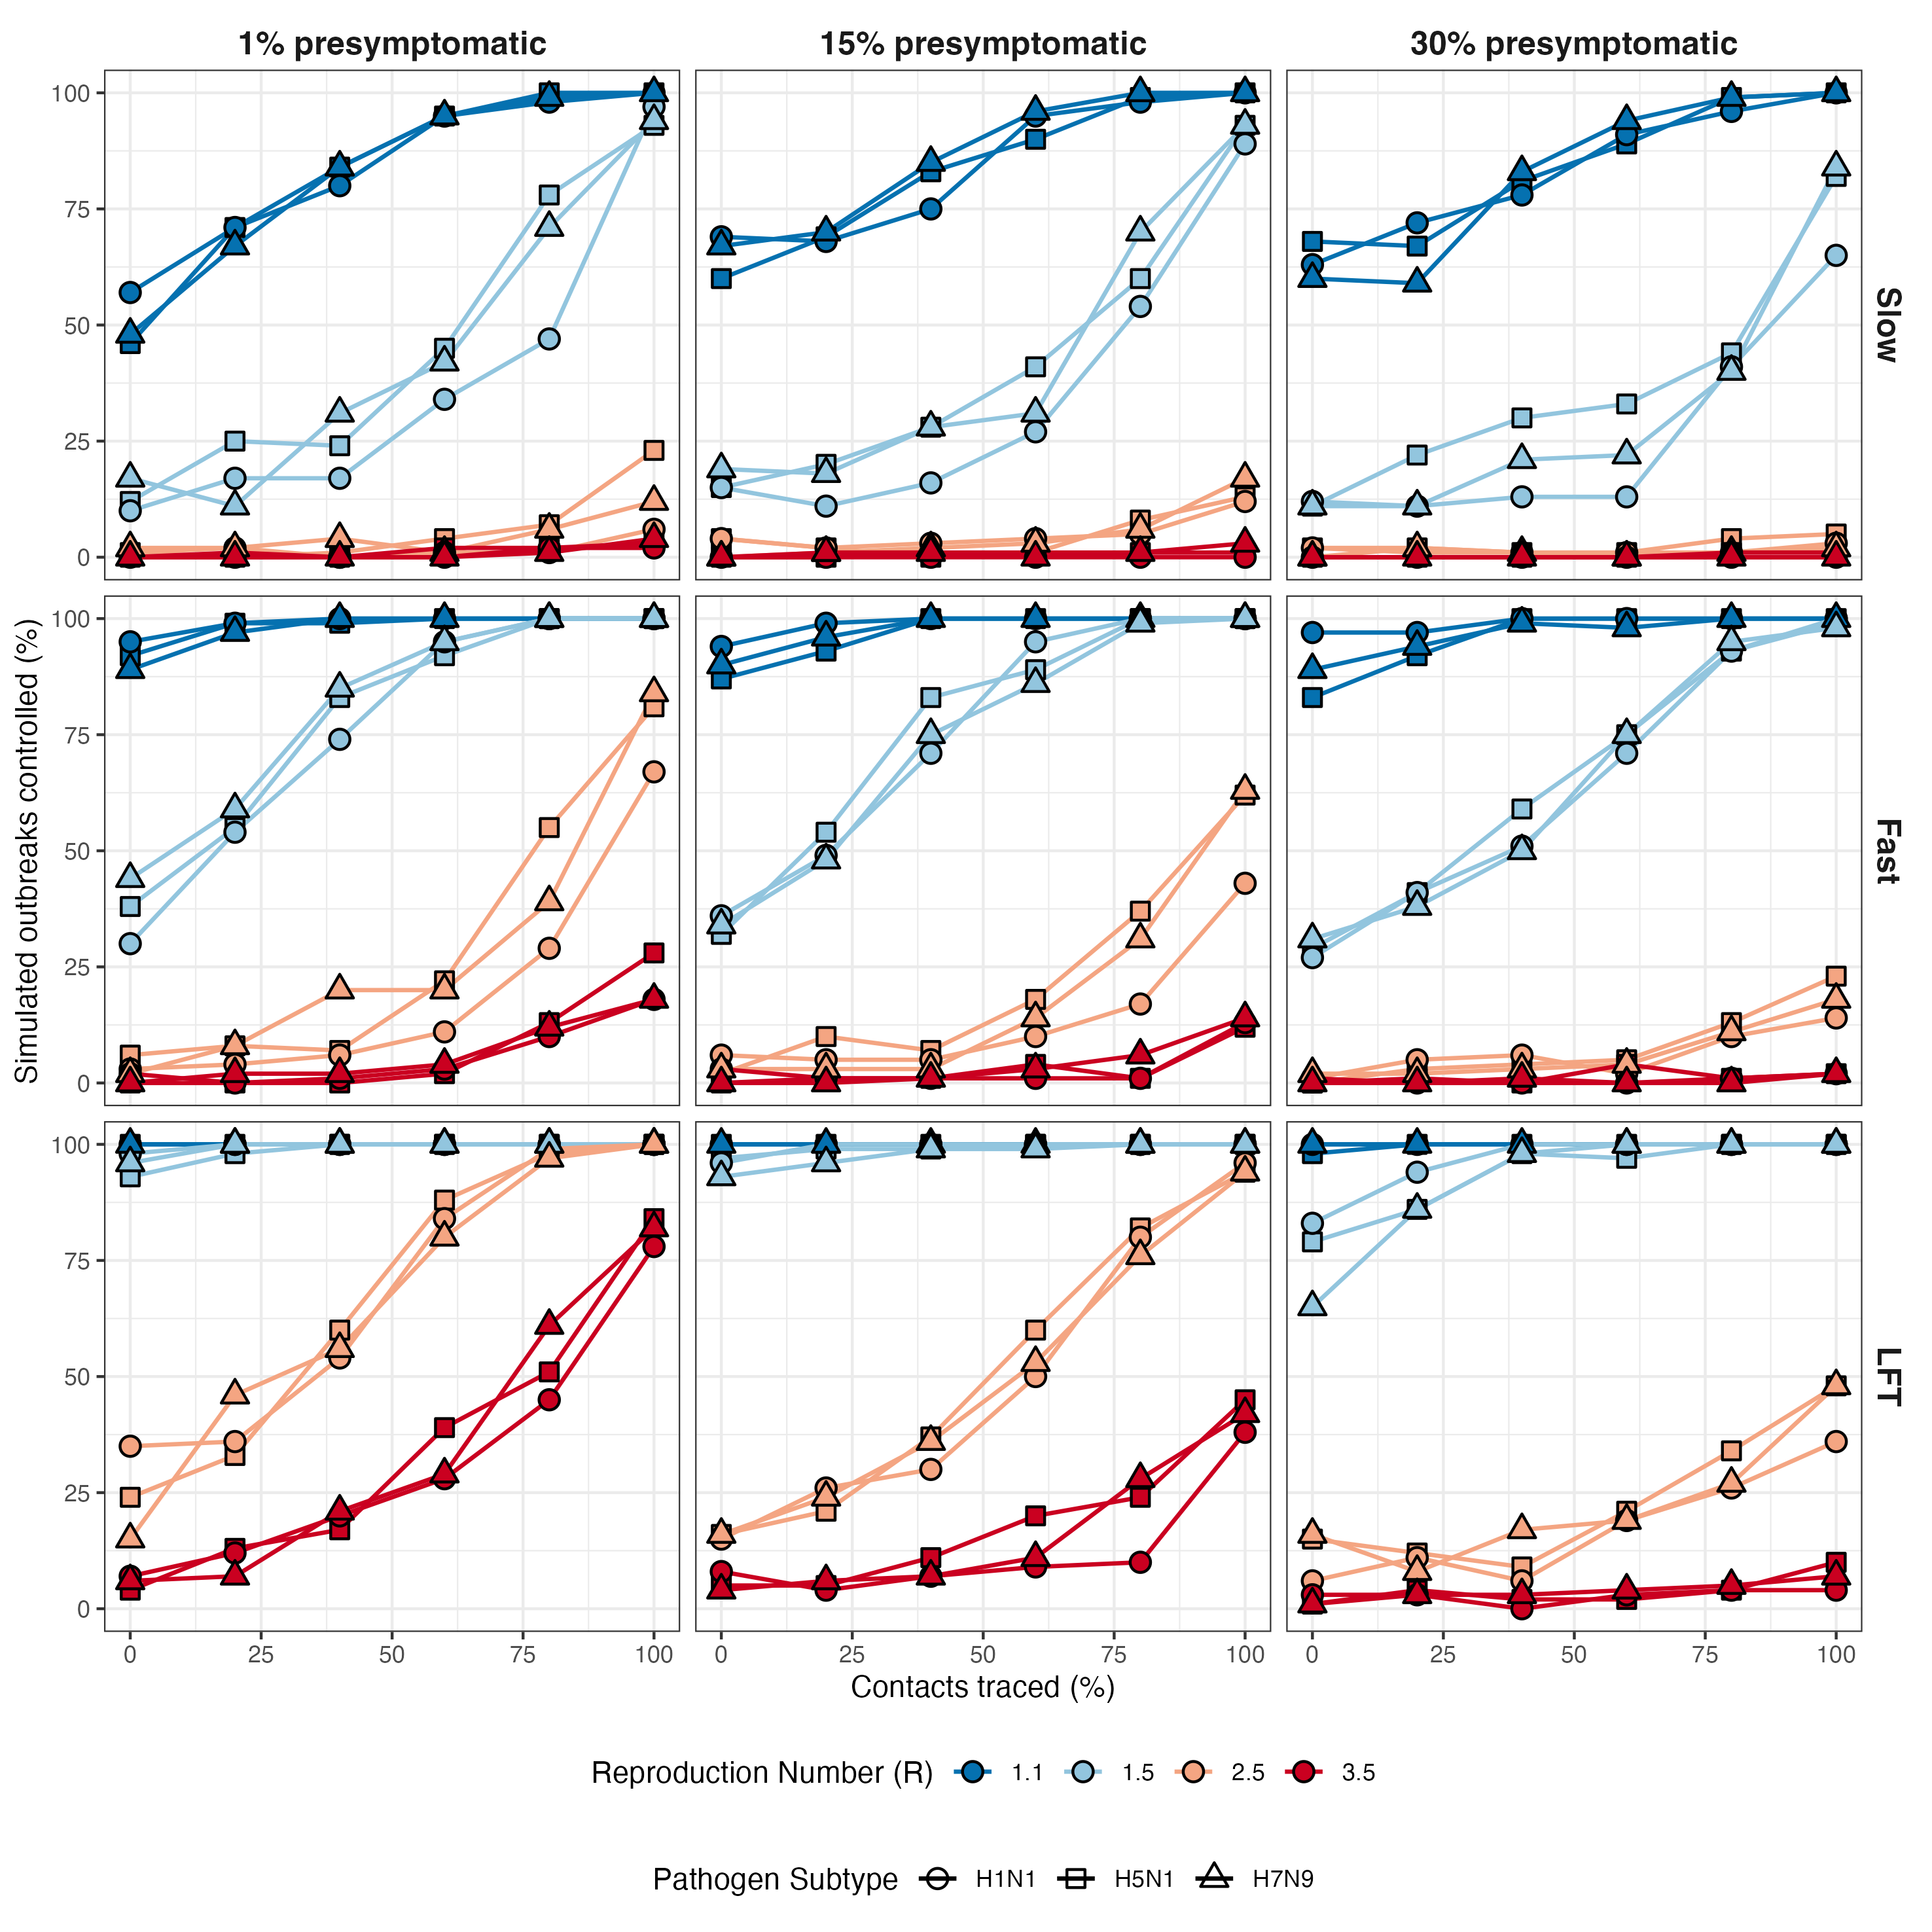
\includegraphics[width=\textwidth]{../plots/prop_outbreak_control_prop_presym_iso.png}
\caption{Stub.}
\label{fig:prop-outbreak-control-prop-presym-iso}
\end{figure}

\begin{figure}[ht]
\centering
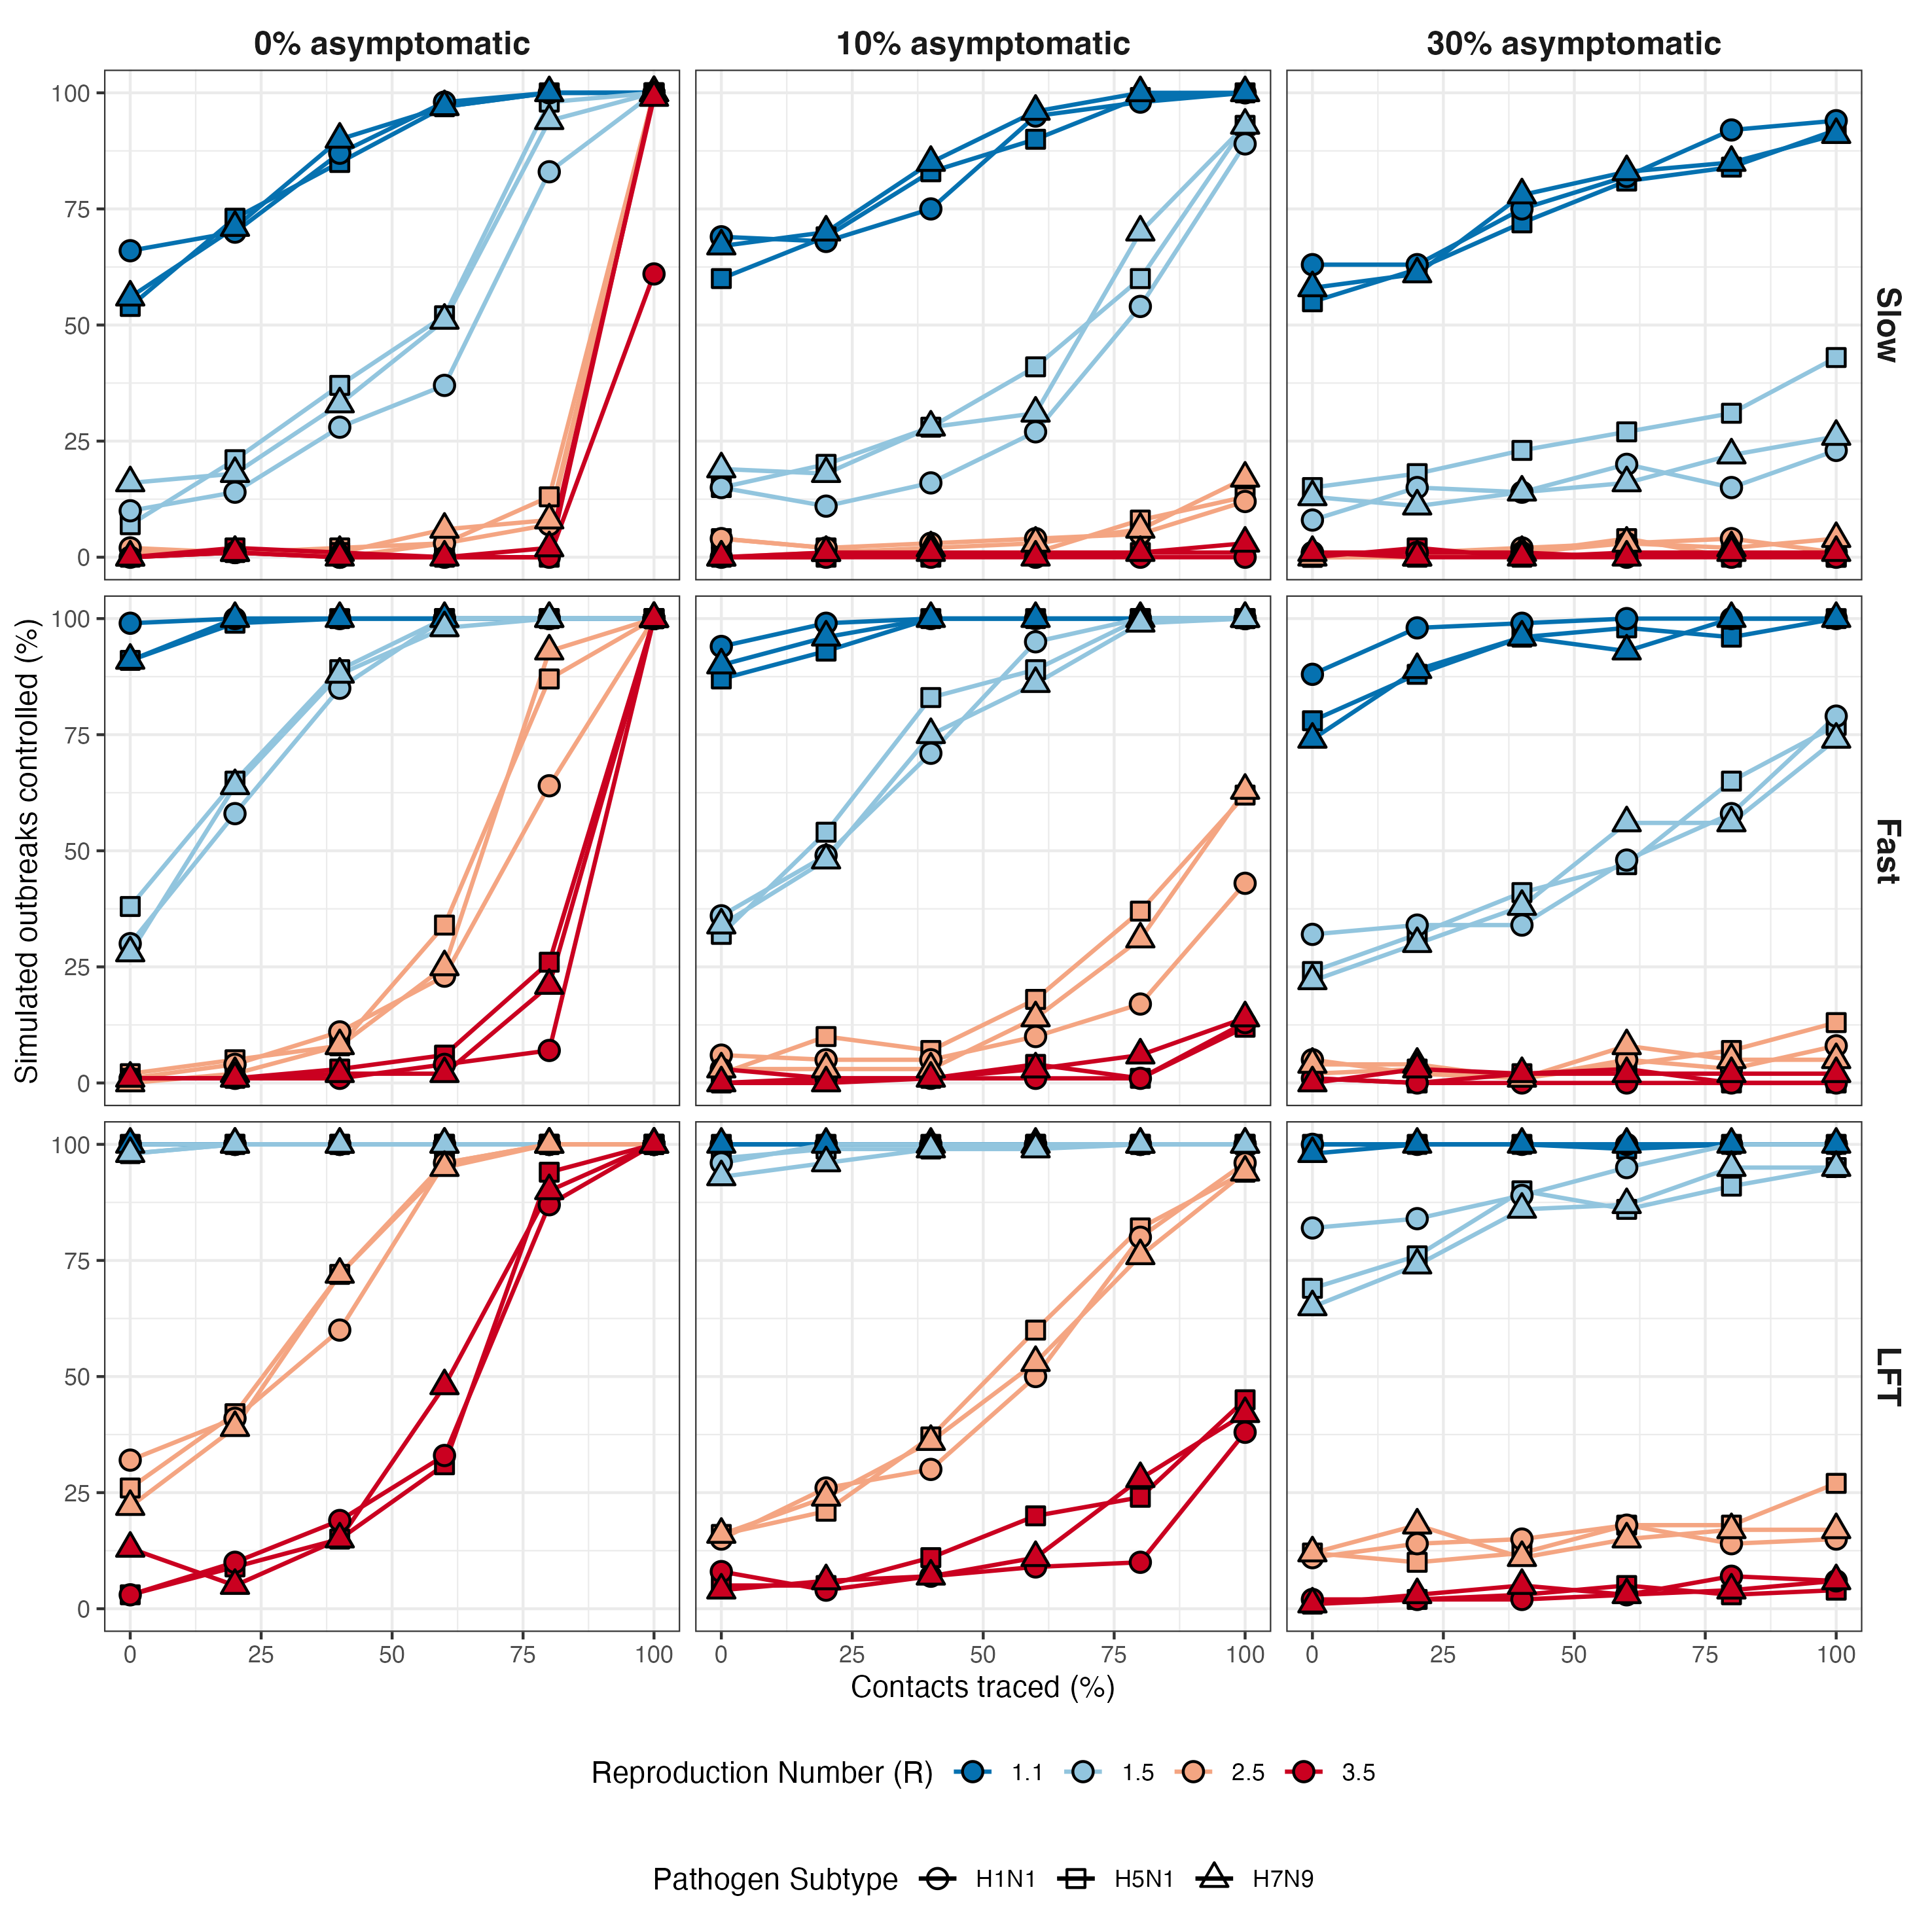
\includegraphics[width=\textwidth]{../plots/prop_outbreak_control_prop_asym_iso.png}
\caption{Stub.}
\label{fig:prop-outbreak-control-prop-asym-iso}
\end{figure}

\begin{figure}[ht]
\centering
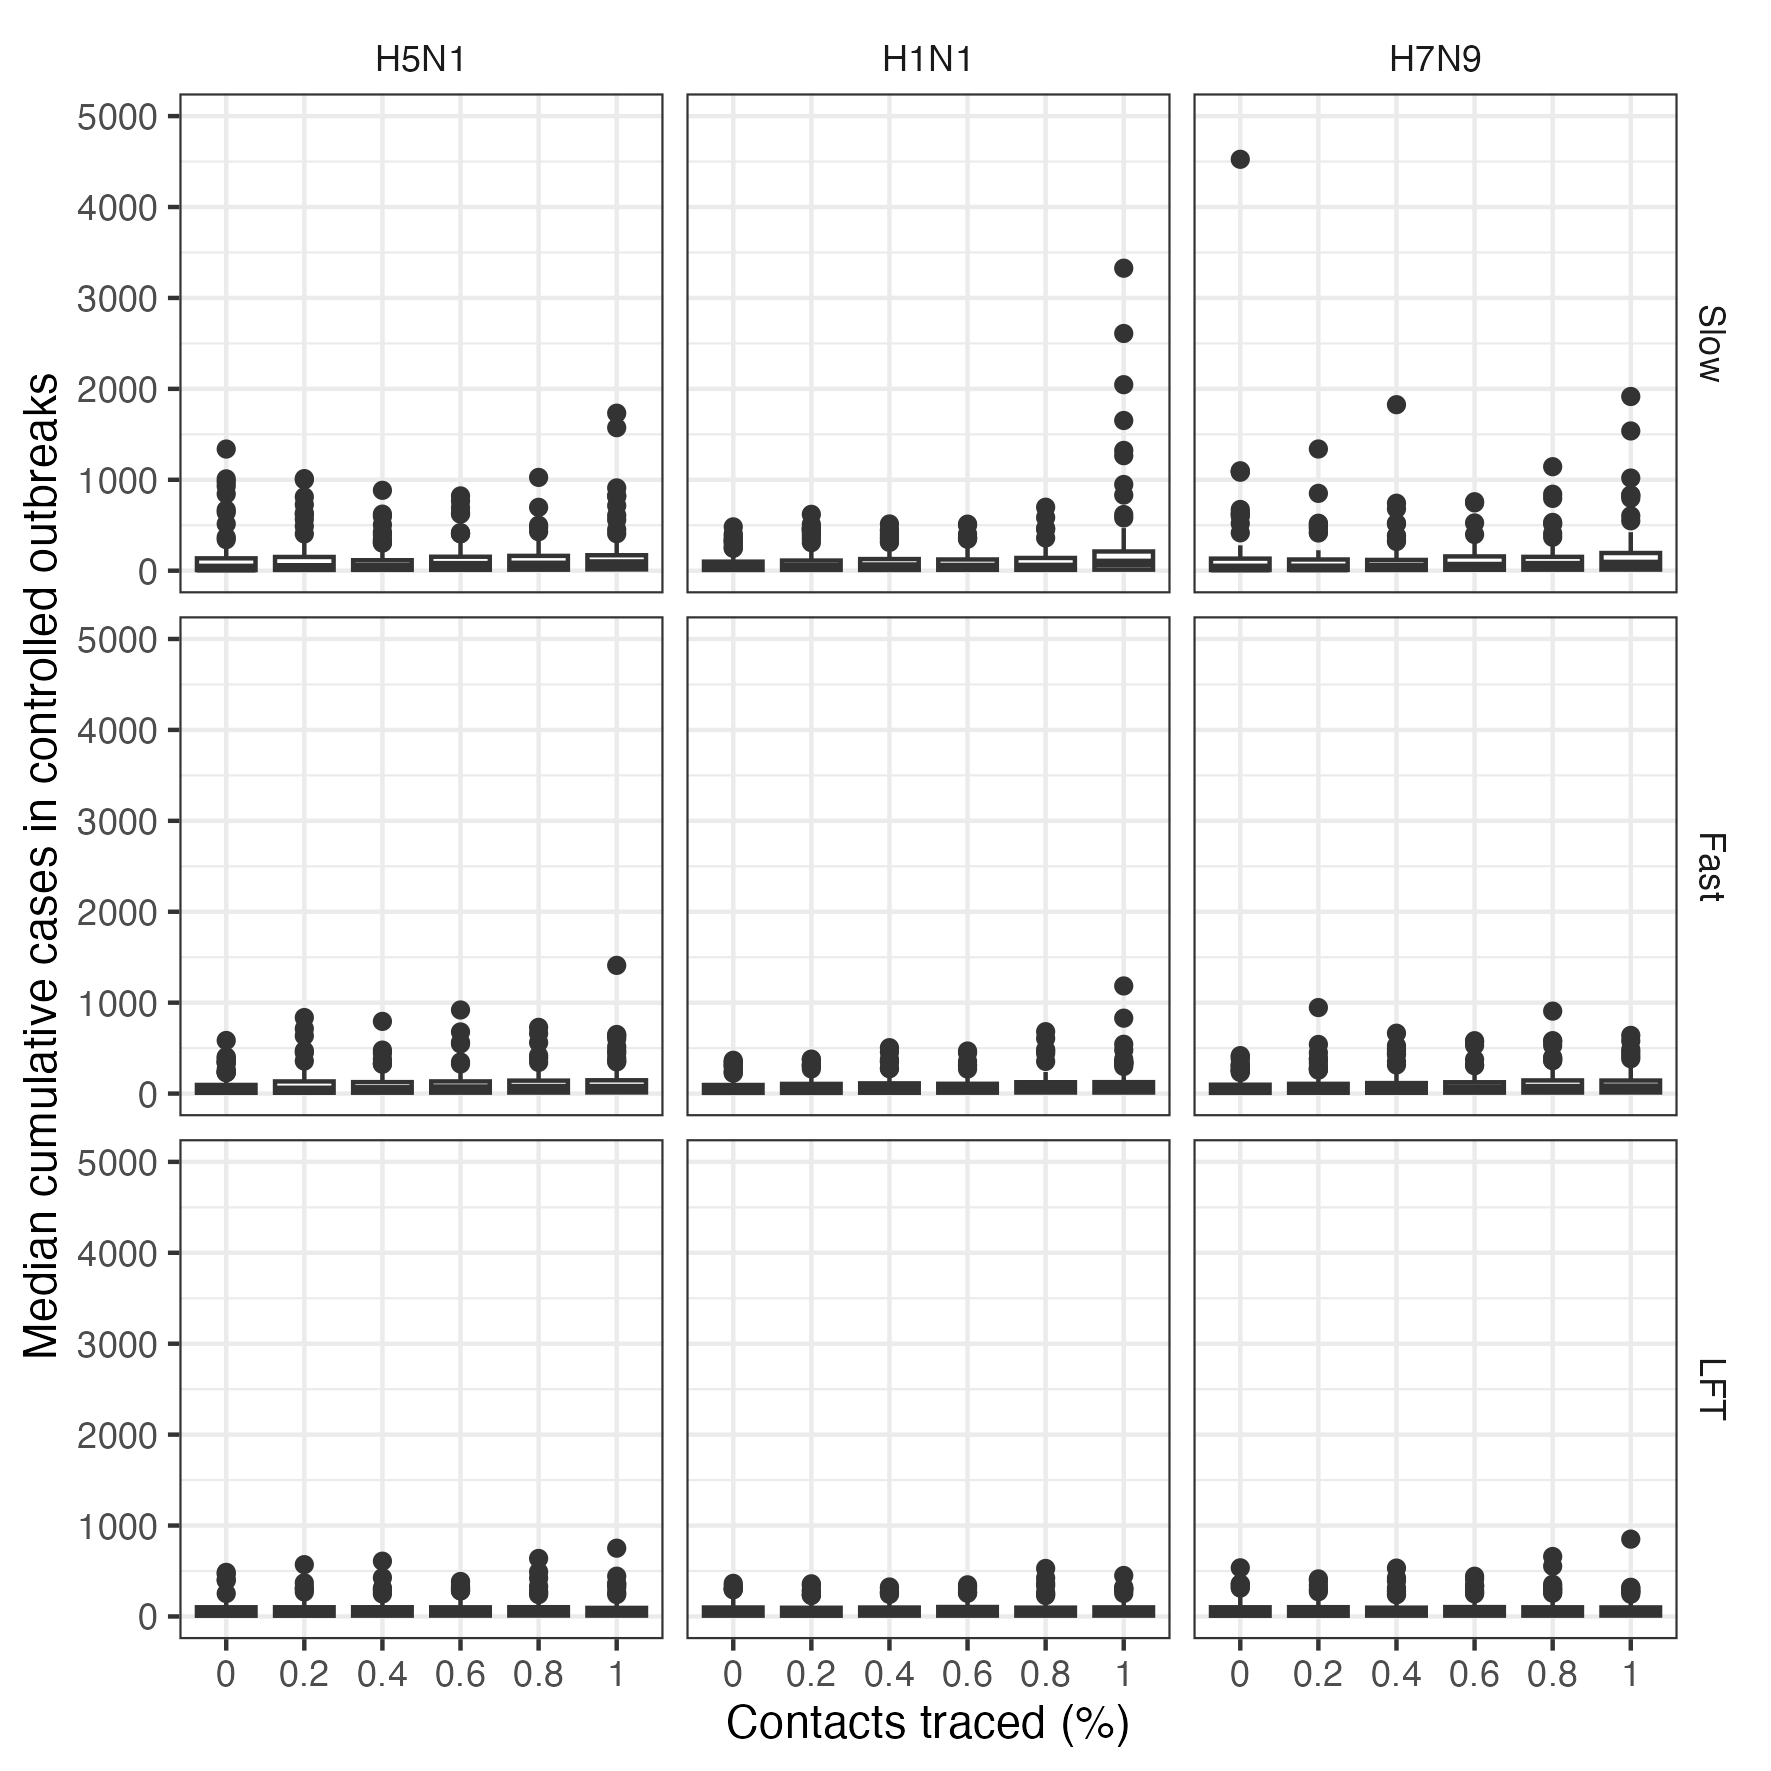
\includegraphics[width=\textwidth]{../plots/median_controlled_outbreak_size.png}
\caption{Median...}
\label{fig:median-controlled-outbreak-size}
\end{figure}

\begin{figure}[ht]
\centering
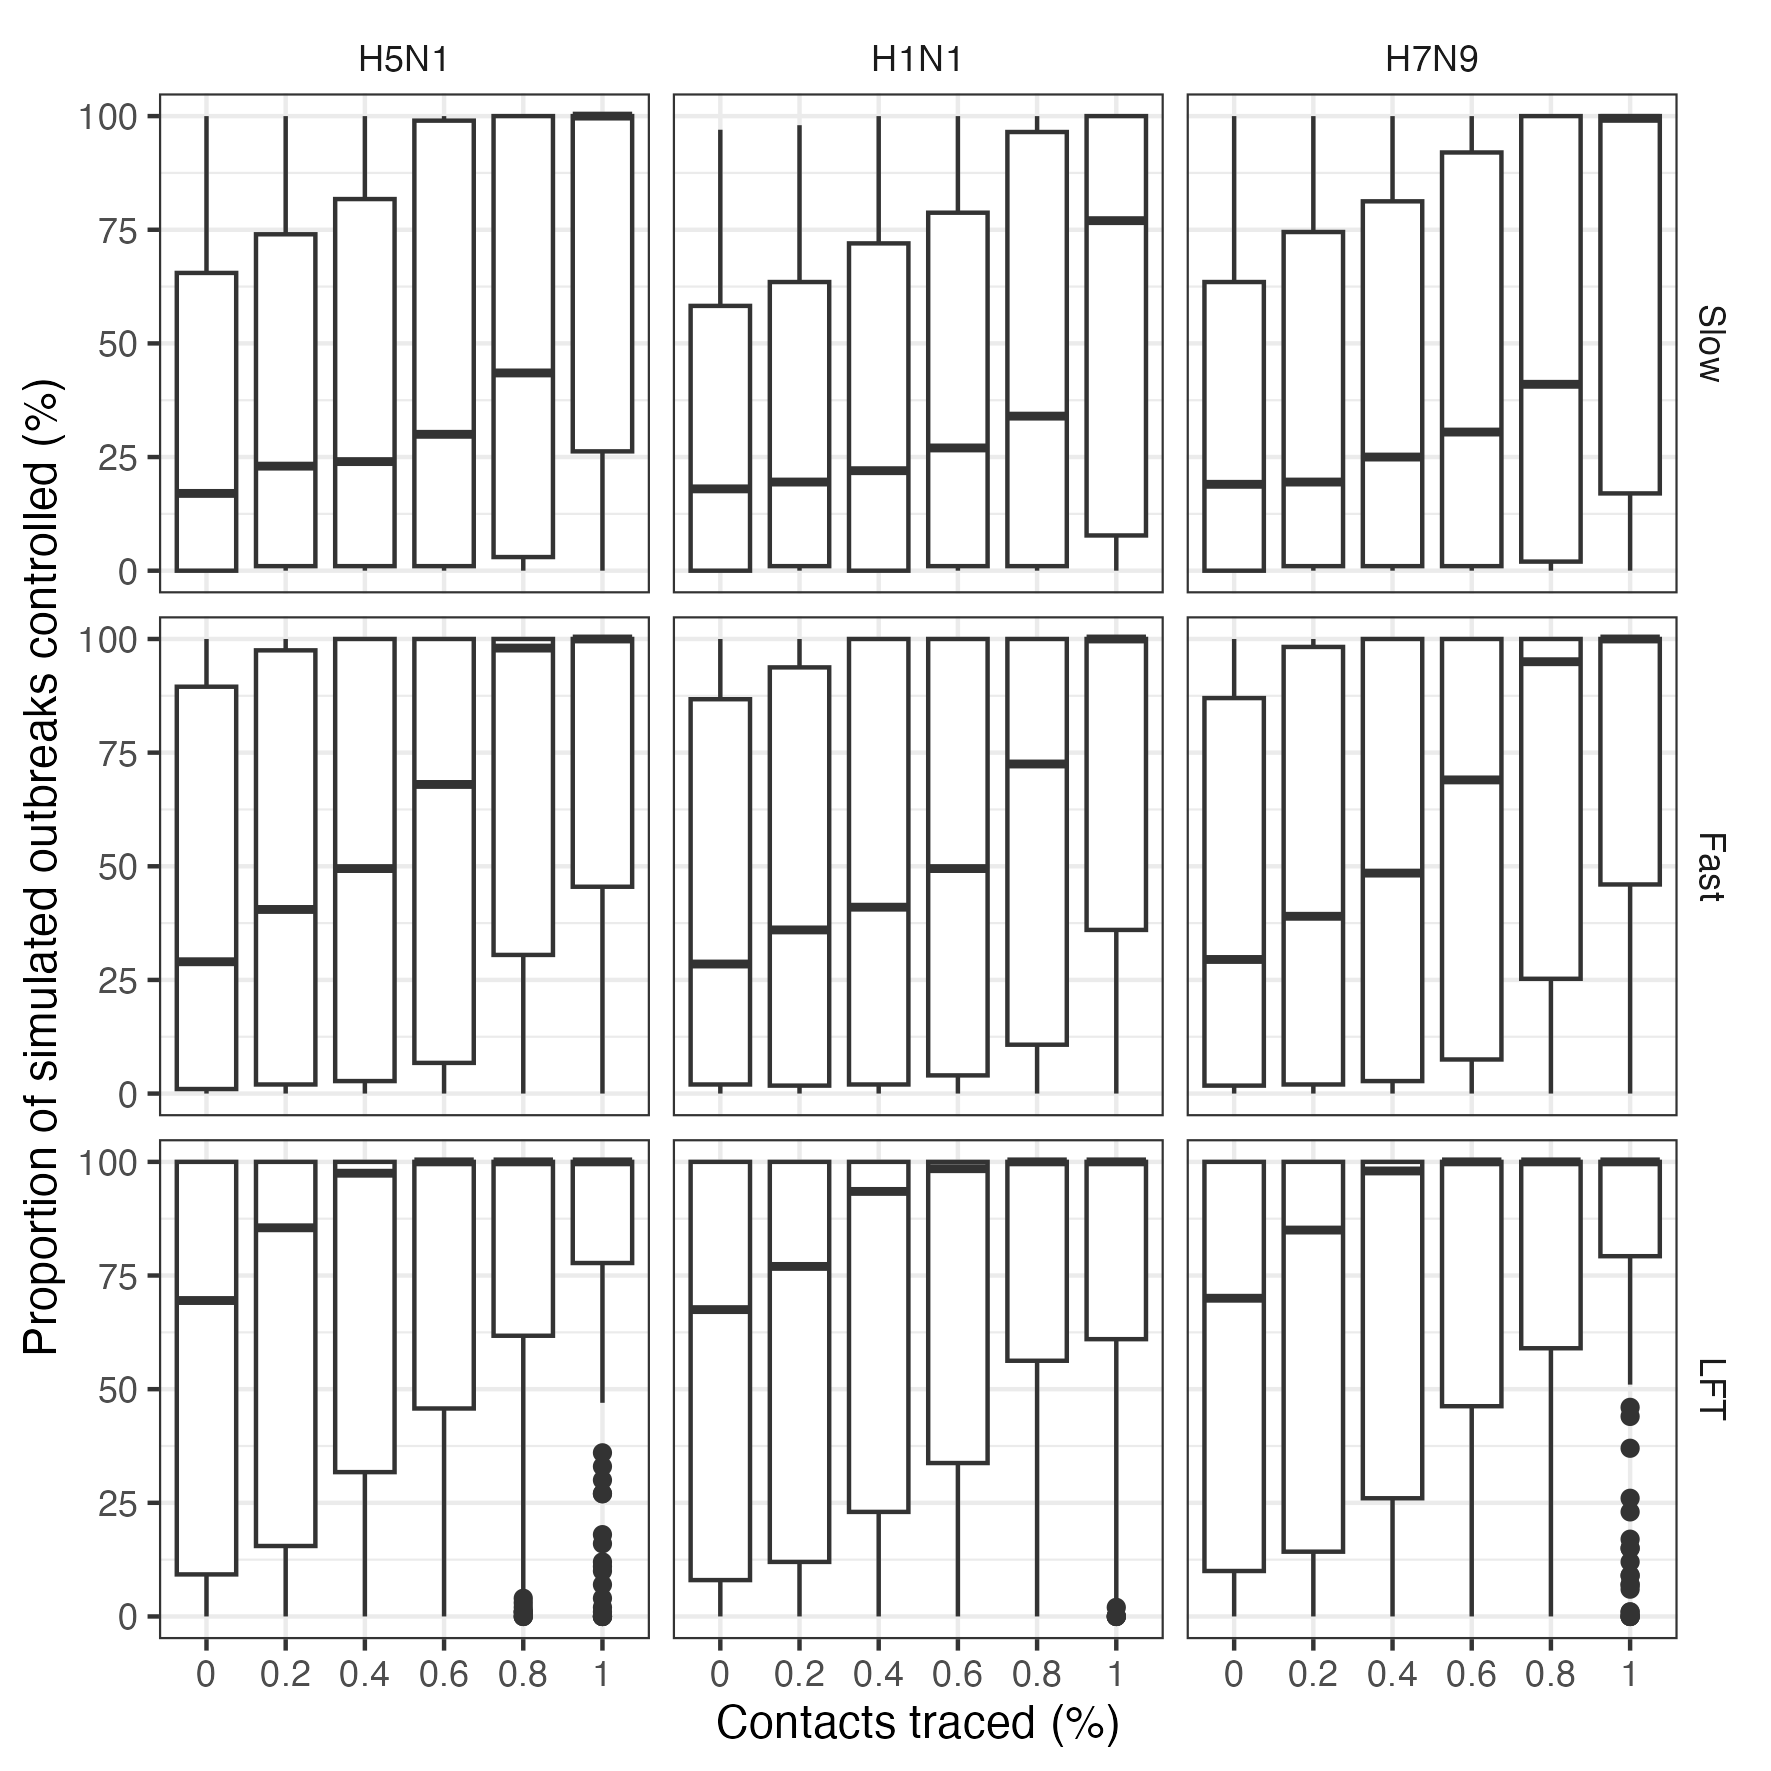
\includegraphics[width=\textwidth]{../plots/prop_controlled_outbreak.png}
\caption{Median...}
\label{fig:prop-controlled-outbreak}
\end{figure}

\begin{figure}[ht]
\centering
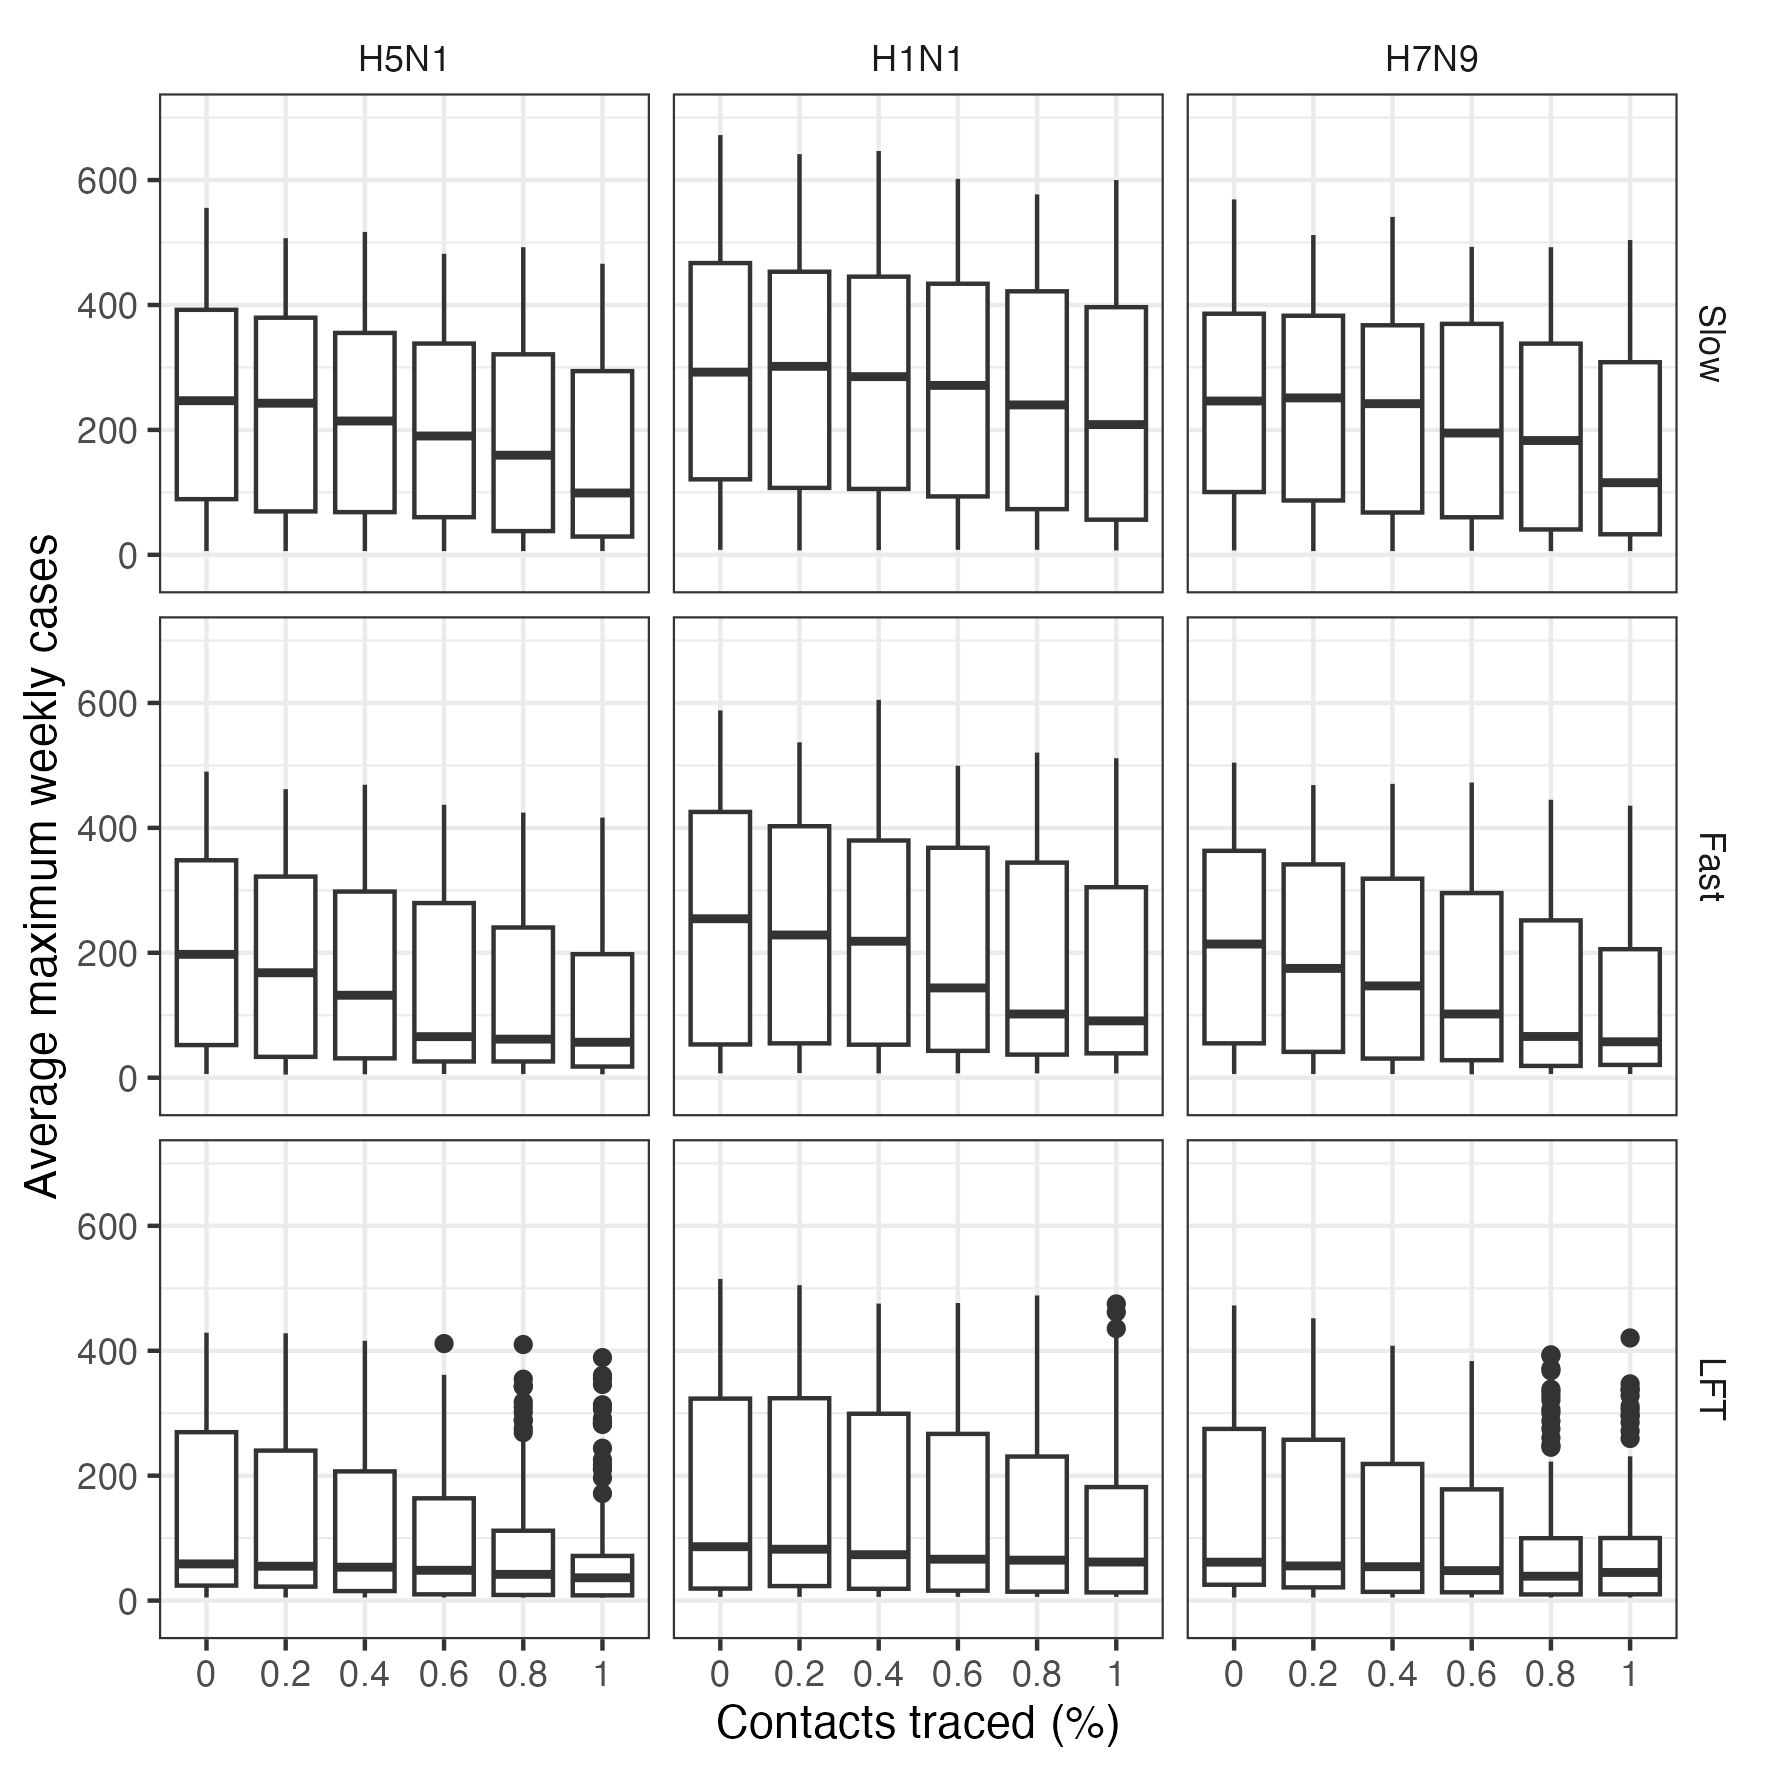
\includegraphics[width=\textwidth]{../plots/max_weekly_cases.png}
\caption{Max...}
\label{fig:max-weekly-cases}
\end{figure}

\end{document}
